%	----- PACKAGES AND OPTIONS ----- 
\documentclass[11pt,a4paper,english,oneside]{article}
\usepackage{etex} %Because of many packages --> Extended TeX.
\usepackage[left=1in, right=1in]{geometry} %Helps to structure the paper layout.
\usepackage[Lenny]{./style/fncychap} %Design of the thesis.
\usepackage[utf8]{inputenc} %Due to vowels.
\usepackage[british]{babel} %Define the language style.
\usepackage{dsfont} %Nice style for the indicator function.
\usepackage{fancyhdr} %To customize the headers and footers.
\usepackage{booktabs} %In case you need \cmidrule or \addlinespace in tables.
\usepackage[hang,bottom,stable,multiple]{footmisc} %Style of footnotes.
%\usepackage{appendix} %For the \appendixpage command.
\usepackage[titletoc,toc,page]{appendix}
%Load some mathematical packages.
\usepackage{amsmath}
\usepackage{amsfonts}
\usepackage{amsmath}
\usepackage{amssymb}
\usepackage{mathtools}
\usepackage[sort,round]{natbib} %For the bibliography.
\usepackage{etoolbox} %To remove the page number on \appendixpage.
\usepackage{amsthm} %For theorems, definitions etc.
\usepackage{thmtools} %For theorems, definitions etc.
\usepackage{setspace} %Use double spacing.
\usepackage{lipsum} %For the \lipsum command to generate a text.
\usepackage{datetime} %For the specification of the date.
%\usepackage{tocloft} %The ToC, LoF and LoT each appear not necessarily on a new page.
\usepackage{graphicx,listings,xcolor,textcomp} %For the graphics, listings etc.
% \usepackage[justification=raggedright,singlelinecheck=true,
%              font=small, labelfont=bf]{caption} %Customize the captions.
\usepackage{caption,threeparttable}
\captionsetup{labelfont=bf,
              justification=raggedright,
              singlelinecheck=false,
              labelfont=bf,
              font=small}
% \usepackage[justification=raggedright,
%             singlelinecheck=false,format=plain]{subcaption}
\usepackage{chngcntr} %To use counterwithout.
\usepackage{epstopdf} %For inserting .eps files into the document.
\usepackage{xparse} %Load for \NewDocumentCommand command.
\usepackage{rotating} %To rotate a table.
\usepackage{pdfpages}
\usepackage{array,hhline} %To create tables and matrices.
\usepackage{tabularx} %An extended version of tabular.
% \usepackage{arydshln} %Due to the capability to draw horizontal/vertical dash-lines.
\usepackage{hyperref} %Must be loaded at the end.
\usepackage{cleveref} %For the command \cref, load after hyperref.
\usepackage{makecell}
\usepackage{cellspace}
\setlength\cellspacetoplimit{4pt}
\setlength\cellspacebottomlimit{4pt}

\graphicspath{ {./../resources/figures/} } %  Figures directory

\renewcommand{\appendixpagename}{\appendixname}
\renewcommand{\appendixtocname}{\appendixname}

\noappendicestocpagenum

%Setup of the reference links.
\hypersetup{
     colorlinks=false,
     linkcolor=blue,
     citecolor=blue,
     filecolor=magenta,
     urlcolor=blue}

%Define some reasonable margins.
\setlength{\textwidth}{6.6in}
\setlength{\textheight}{8.8in}
\setlength{\topmargin}{-0.1in}
\setlength{\oddsidemargin}{0in}
\setlength{\parskip}{1mm}

\bibliographystyle{abbrvnat} %Reference style.
\allowdisplaybreaks[1] %Page breaks of equations are allowed, but avoided if possible. 2-4 more relaxed.

%New command for the UZH logo.
\newcommand*{\plogo}{
\includegraphics{./style/uzh_logo_e_pos}}

%New command for the differential d to have an ordinary d.
\makeatletter
  \newcommand{\ud}{\mathrm{d}}
\makeatother

%Remove page number on \appendixpage. Use the package 'etoolbox'.
\makeatletter
\patchcmd{\@chap@pppage}{\thispagestyle{plain}}{\thispagestyle{empty}}{}{}
\makeatother

%Declare Definitions, Theorems etc.

%Readjust the numbering.
%\counterwithout{footnote}{chapter}
%\numberwithin{equation}{chapter}

\setlength{\parindent}{0cm} % Uncomment this if you don't want to have indents.

%	----- TITLE PAGE ----- 
\newcommand*{\titleGP}{\begingroup %Create the command for including the title page in the document.
\centering %Center all text.
\vspace*{\baselineskip} %White space at the top of the page.
\plogo\\[2\baselineskip] %University Logo.
\rule{\textwidth}{1.6pt}\vspace*{-\baselineskip}\vspace*{2pt} %Thick horizontal line.
\rule{\textwidth}{0.4pt}\\[\baselineskip] %Thin horizontal line.
{\LARGE Scarcity channel of Quantitative Easing :}

\vspace*{3pt}

{\LARGE Examining the Overnight Treasury Repo Market in the US}\\[0.2\baselineskip] %Title.
\rule{\textwidth}{0.4pt}\vspace*{-\baselineskip}\vspace{3.2pt} %Thin horizontal line.
\rule{\textwidth}{1.6pt}\\[2\baselineskip] %Thick horizontal line.
\scshape %Small caps.
Master's Thesis\\[2\baselineskip]
Submitted in partial fulfillment of the requirements for the degree of Master of Arts in Economics and Business Administration \par
\vspace*{2\baselineskip}
Author\\
{\Large Hubert Mrugala \\ [5pt]
 }
Seemattweg 4, 6315 Oberageri \\[5pt]
19-764-265 \\[5pt]
hubert.mrugala@uzh.ch \\


\vspace*{2\baselineskip}
Supervisor\\
{\Large Prof. Dr. Kjell Nyborg\\[5pt]\small Chaired Professor of Finance\\[5pt]
\small Department of Banking and Finance\\[5pt]University of Zurich\par}
\vspace*{2\baselineskip}
Assistant\\
{\Large Benjamin Schneider \par}
\vfill
{\scshape Date of Submission: \textcolor{red}{DRAFT}} \\[0.3\baselineskip] % 18.05.2022
\endgroup}

% ----- SPECIAL HEADER AND FOOTER STYLE  ----- 
% for the executive summary and Task Assignment section.
\fancypagestyle{firststyle}{%
  \fancyhf{}%
  \renewcommand{\headrulewidth}{0pt}
  \fancyfoot[C]{\thepage}}

%Customize headers and footers.
\pagestyle{fancy}
\fancyhead[R]{\thepage}
\fancyhead[L]{\rightmark}
\fancyfoot[L]{Hubert Mrugala}
\fancyfoot[C]{}
\fancyfoot[R]{Scarcity channel of Quantitative Easing}

%Define the signature line with dots.
\NewDocumentCommand \dotbox {o O{.5\linewidth} m O{3ex} O{\linewidth}}
{
  \begin{minipage}{7cm}
    \makebox[7cm][l]{\,.\dotfill}
    \\
    \makebox[7cm][l]{\,#3}
  \end{minipage}
}

% ----- BEGIN DOC AND PROJECT DEFINITION ----- 
\begin{document}

\thispagestyle{empty}
\titleGP
\newpage
\doublespacing
\setcounter{page}{1}
\pagenumbering{Roman}
\section*{Task Assignment}

\begin{figure}[h!]
  \begin{center}
    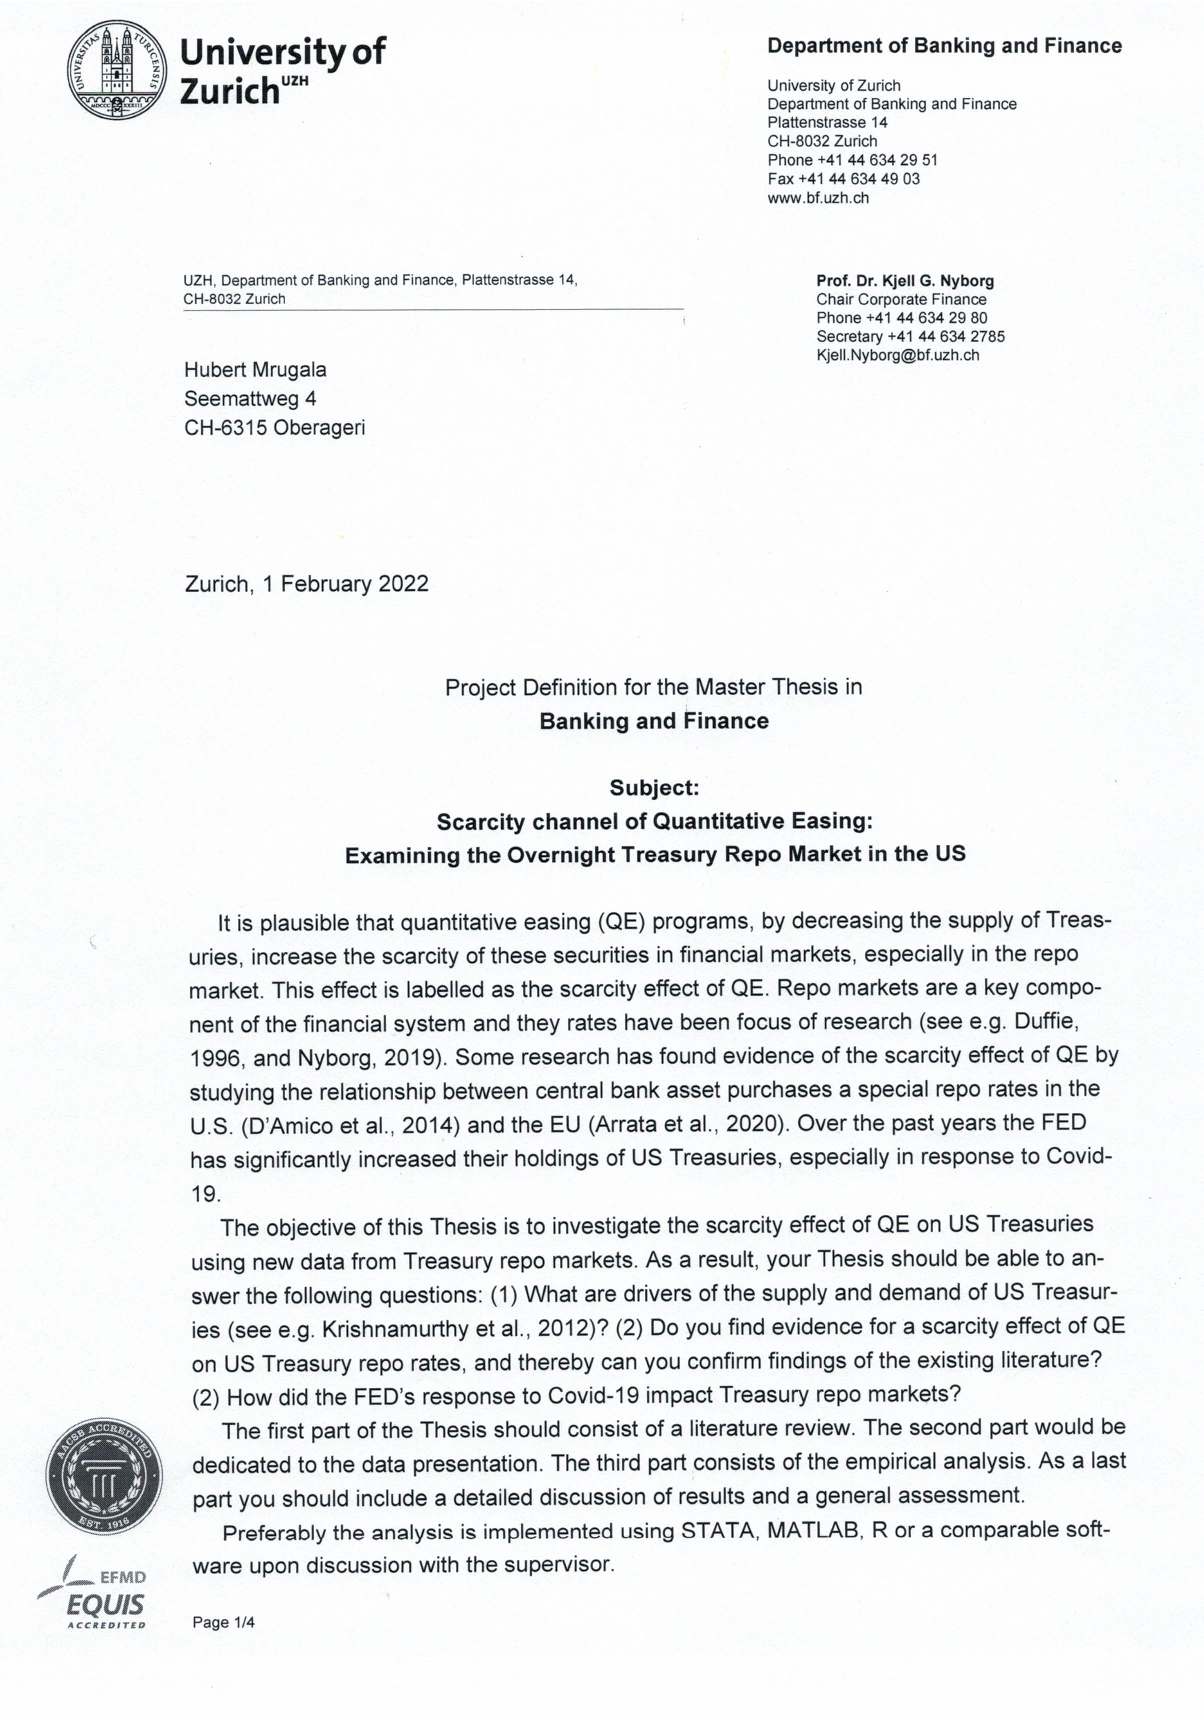
\includegraphics[page=1,width=.86\textwidth]{../../project_definition.pdf}
  \end{center}
\end{figure}
\newpage
\begin{figure}[h!]
  \begin{center}
    \includegraphics[page=2,width=.86\textwidth]{../../project_definition.pdf}
  \end{center}
\end{figure}
\newpage
\begin{figure}[h!]
  \begin{center}
    \includegraphics[page=3,width=.86\textwidth]{../../project_definition.pdf}
  \end{center}
\end{figure}
\newpage
\begin{figure}[h!]
  \begin{center}
    \includegraphics[page=4,width=.86\textwidth]{../../project_definition.pdf}
  \end{center}
\end{figure}

\thispagestyle{firststyle}
\newpage

% ----- EXEC SUMMARY AND ABSTRACT ----- 
\section*{Executive Summary}
\thispagestyle{firststyle}

\lipsum[1-3] % Here goes the text

\newpage
\tableofcontents
\newpage
\listoffigures
\listoftables
\newpage
\pagenumbering{arabic}

\begin{center}
  {\Large \emph{\textbf{Scarcity channel of Quantitative Easing:\\
  Examining the Overnight Treasury Repo Market in the US}}}\\[4pt]
  Hubert Mrugala
\end{center}

\abstract{\lipsum[1]}

\begin{flushleft}
  \textbf{JEL classification}: E4, E5\\
  \textbf{Keyword}: Collateral, Scarcity, Treasury, Monetary Policy, Repo Market
\end{flushleft}

% ----- INTRODUCTION ----- 
\section{Introduction} \label{sec:introduction} % 3.5 - 4 pages

The COVID-19 pandemic has caused the deepest US recession since the Great Depression and induced the biggest monetary stimulus since the Global Financial Crisis. One of the monetary policy tools that was activated during the pandemic was an additional round of quantitative easing.\footnote{It was actually an acceleration of already present QE that was sparked by 2019 repo rumble.} In the time of 4 months, the Fed's balance sheet exploded from \$4.2 to \$7.1 trillion, and then kept growing. As of April 2022, total assets of the Fed reached almost \$9 trillion. Central bank asset purchases are used in normal times as a unconventional policy that helps achieving ultimate goals of the Fed, which are maximum employment and inflation level at 2\% over the longer run.

There are many theoretical transmission channels of quantitative easing, however almost all of those channels focus on positive effects of asset purchases. Negatives are very rarely analysed. \citet{nyborg2015} showed that collateral frameworks of ECB distort financial markets' efficiency by making bad collateral look better then it really is. What about a high-quality collateral? Can draining fist-class collateral out of the markets have an adverse impact on the economy?

There is one channel of quantitative easing that is rarely mentioned and insuffitiently studied.\footnote{In financial media, only Izabella Kaminska of FT Alphaville sometimes covered collateral scarcity.}. It is the scarcity channel (or scarcity effects). While most channels on QE focus on abundance of reserves, central bank liquidity, the scarcity effect, puts emphasis on the collateral-side of the swap, which is the public sector liquidity. There are only two academic papers that study the scarcity channel of asset purchases programmes. \citet{damico2014} find that there was a scarcity premium of US Treasury securities traded in the repo market during the time of LSAP programs. Likewise, \citet{arrata2018} determine a similar relationship in the \textbf{Euro zone market for repo contracts}. Both papers prove the existence of the scarcity effects in the US and EU markets, however, those investigations look only at specific special repo markets and don't take into account the mechanics of the collateral intermediation complex. Furthermore, there hasn't been any research done about the scarcity premium of US Treasuries in over eight years, despite an almost constant QE during that period.

This research fills the subject gap, the time gap, and the context gap in the narrow literature on scarcity effects. I use a General Collateral Financing Treasury Repo rate weighted index in a timespan of the last 15 years to test a connection between the level of US Treasury securities on the Fed's balance sheet and the index. Additionally, to focus completely on the collateral-side of a repo transaction, I use a collateral spread as the dependent variable. \citet{nyborg2019b} \textbf{find ...}

\textbf{[Findings]}

I control for \textbf{[...]} and emphasize the importance of high-quality collateral by describing its dynamics and economic function. Moreover, I add an innovative proxy for the re-use rate of collateral in the banking system as an extension of the base model.

The research connects three different strains of literature, which are research on collateral scarcity, US Treasury markets and collateral intermediation.

Apart from already mentioned academic papers on scarcity effects, there is also one investigation of the Japanse JGB market that contributes to the literature on collateral scarcity. \citet{han2018} have documented that BoJ purchases of Japanese Government Bonds in QE and then QQE programs have negative impact on market liquidity, which suggest scarcity effects.

The second stain is the literature on repo market rates and cash market rates of US Treasuries. The work of \citet{duffie1996} introduced a model that shows how short-selling Treasuries obtained by reverse-repo transactions can create squeezes at delivery dates and so, cause some repos to trade on special. Special repo rates are not studied in this research, however, mechanics of special repos are important because US Treasuries, as a whole asset group, are special on their own. \citet{krishnamurthy2012} show that yields of US Treasury securities have a non-default component that makes them trade at a significant premiu. 

The last branch of literature is concerned with the collateral supply and its intermediation. \citet{singh2011} shows how collateral agency is embedded into the shadow banking system. \citet{sissoko2020} show how sufficient collateral supply is crucial to properly functioning money markets and effective monetary policy. \citet{singh2012} introduce and explain a phenomenon of "collateral-chains". \citet{singh2017} calculates the collateral re-use rate that represents endogenous shadow creation of collateral. \citet{jank2021} finds a positive relationship between ECB bond purchases (PSPP) and the re-use rate of collateral suggesting that the market participants adjust to shocks in collateral scarcity by utilizing more source collateral.

Investigating scarcity effects of unconventional monetary policy is important because it is not certain that government bond purchasing programs of central banks have a net positive effect on the real economy. Benefits of QE or PSPP are not clear. Despite over 10 years of bloated central bank balance sheets, inflation and growth did not follow.\footnote{According to \citet{gern2015}, increase in GDP and inflation are two final effects of the QE/PSPP transmission mechanism.}. If scarcity effects are large and significant, then a lack of central bank unsterilized actions in response to an external shock may be more beneficial than active bond purchases. Nonetheless, the final assessment must be made by looking at the bigger picture and taking into account other factors like the regulatory environment and demand for reserves. This work studies only scarcity effects. \textbf{Last but not least, scarcity effects and connection to .. may shed a light on why some central banks decide to apply controvenial collateral frameworks.}

% Figure: Fed's BS
\begin{figure}[htb!]
  \begin{center}
    \caption{The long-term rate has been very low in spite of massive QE}
    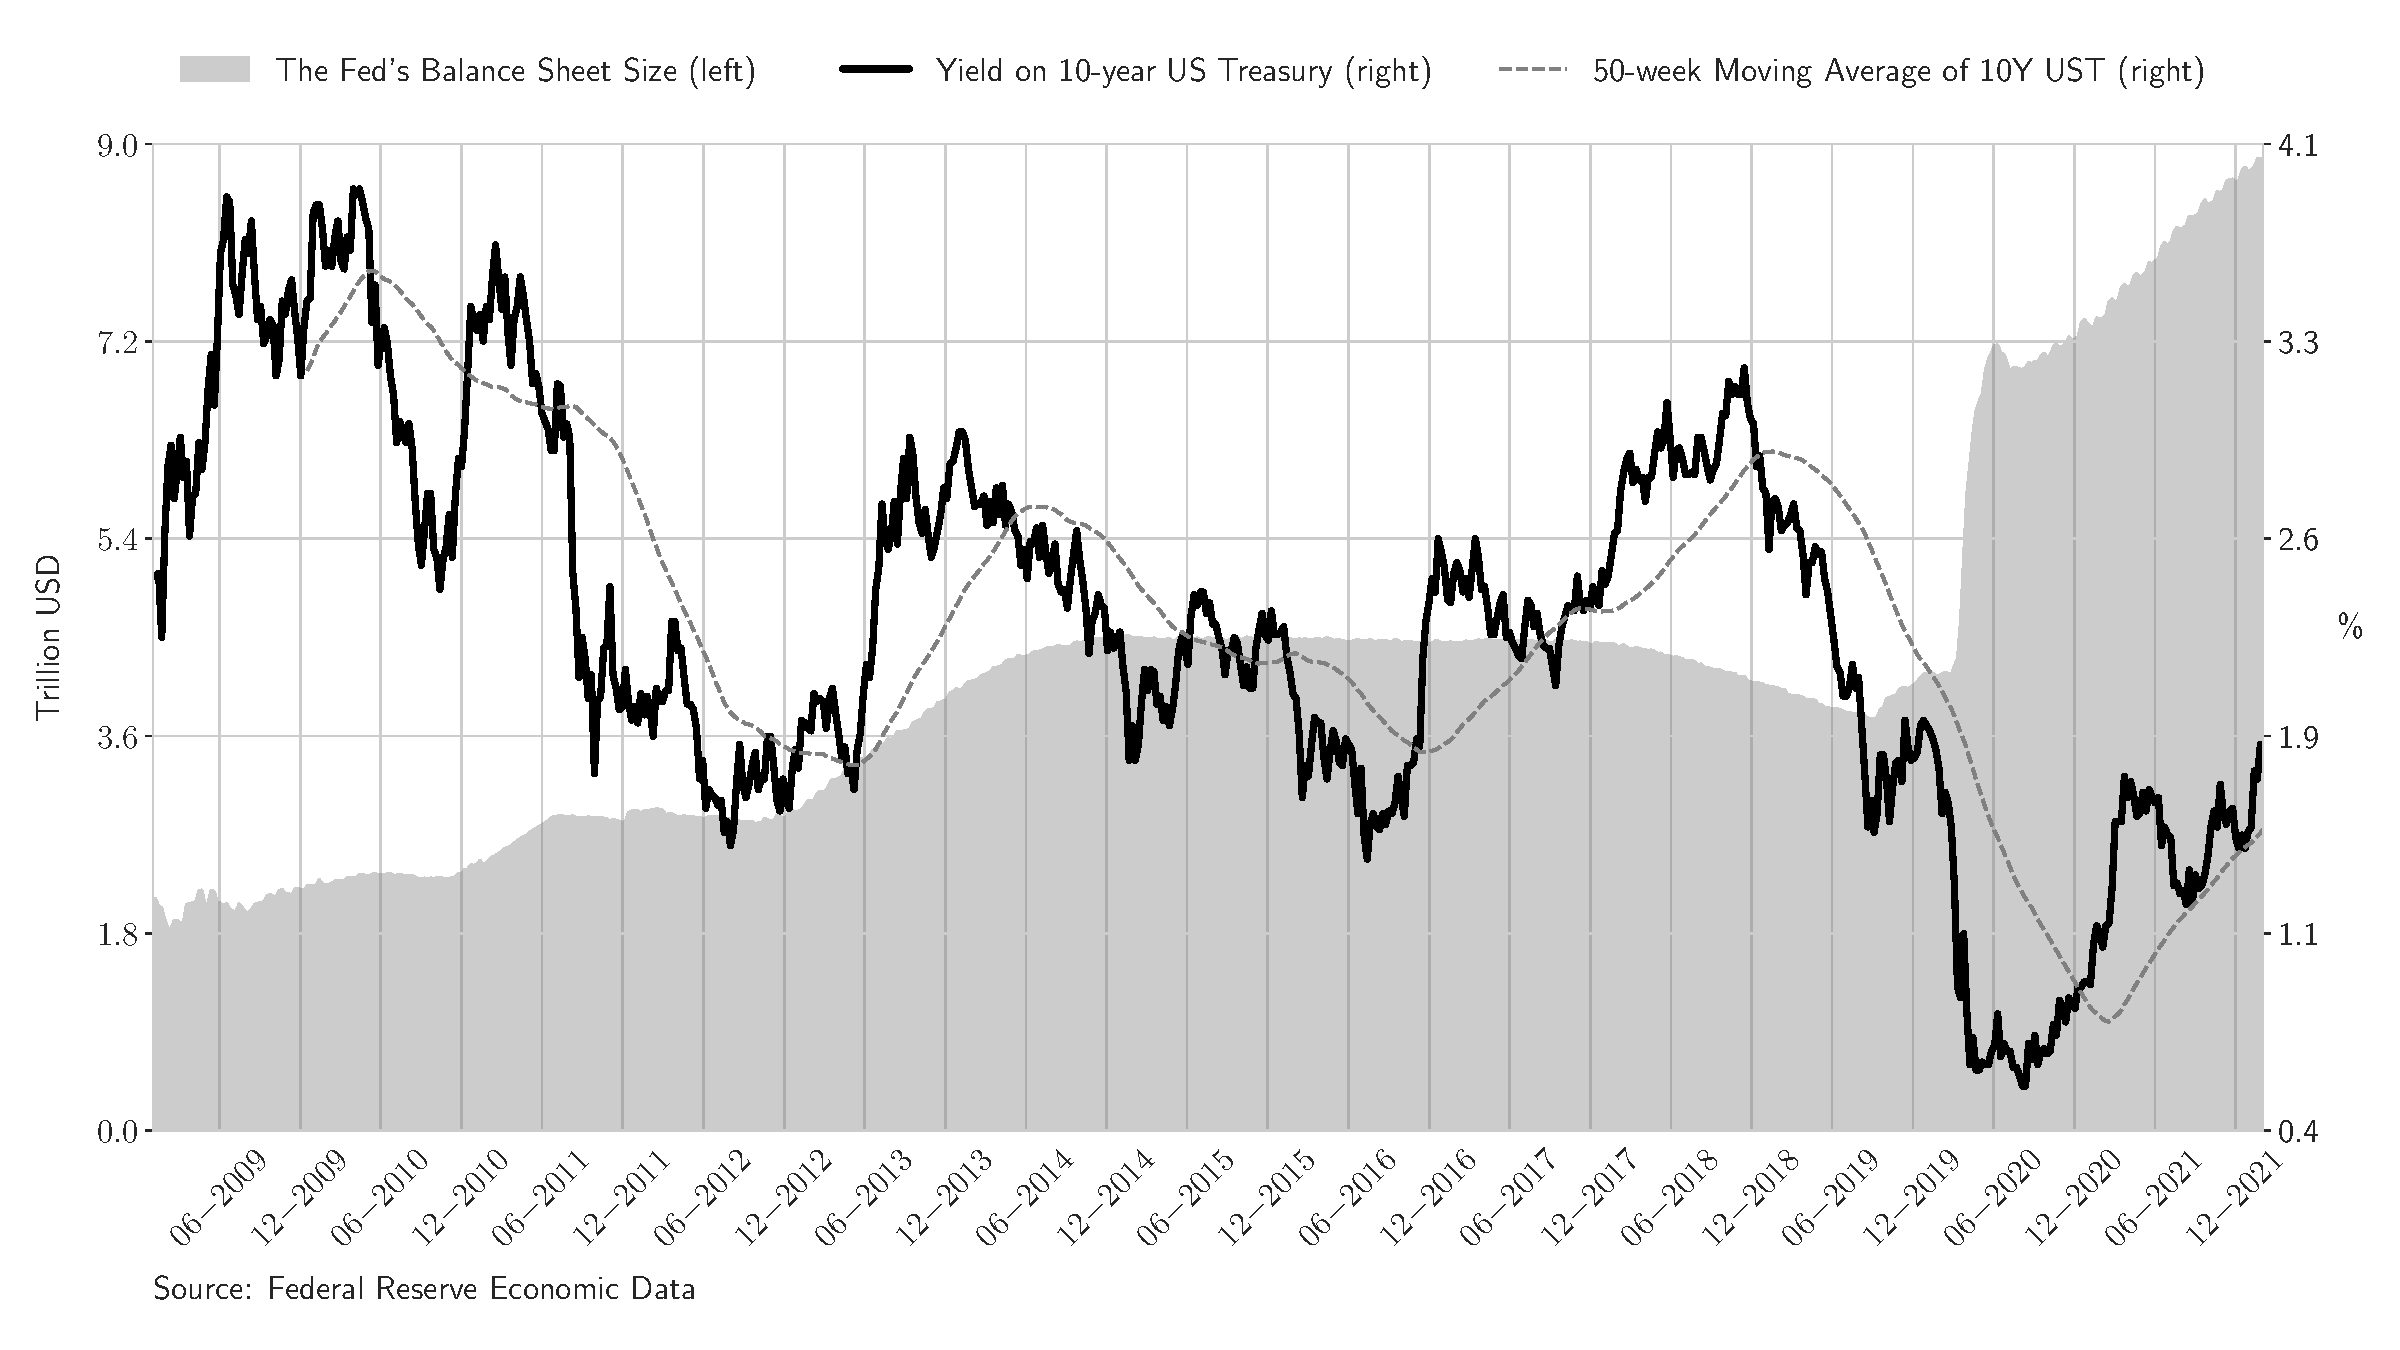
\includegraphics[width=0.99\linewidth]{fed_bs.pdf}
  \end{center}
  \label{Feds_BS}
\end{figure}

The remainder of the paper is organized as follows. \textbf{Section two. Section three.} The last section concludes.

\newpage

% ----- COLLATERAL MECHANICS ----- 
\section{Mechanics of collateral} \label{sec:mechanics}

\subsection{Market for collateral}

Collateral intermediation is facilitated primarily through three kinds of transactions: repo contracts, securities lending and over-the-counter derivative positions. Each of these ways of obtaining collateral is different\footnote{The biggest difference between those instruments, from a point-of-view of the party that receives collateral, is the balance sheet cost of that collateral that is associated with each type of transaction.}, but have one thing in common, which is financial intermediation. Whether the final goal of the counterparty is to secure short-term funding, borrow a security or open a synthetic position, it can be easily done without pledging a very safe and liquid asset in exchange. For this reason, collateral is sometimes referred to as lubrication of the global financial plumbing. It is at the center of the modern money creation process.

The market value of collateral is discounted with a "haircut", that after reduction, yields the maximum value of a loan or a trading position that can be taken. Therefore, the higher the quality of collateral, the higher its utility. The global financial crisis destroyed a large chunk of the private collateral pool, leaving the financial system with public collateral of the most developed economies. According to the 2021 Annual Report to Congress of the Office of Financial Research (OFR), money market funds' (MMF) share of outstanding repo agreements increased from 15.8\% in 2008 to 30.1\% in 2021. On the other hand, MMFs share of commercial paper, during the same time, decreased from 39.5\% to 13.5\%. MMFs are a key provider of short-term funds \citet{ofr2021}.

The main players in the market for collateral are hedge funds, (securities lending) custodians, money market funds, dealers banks and central banks. Hedge funds and securities lenders provide collateral, which then goes through primary dealers to money market funds and commercial banks \citet{singh2017}.

Primary dealers are especially important in the collateral intermediation network, because of their function as a liaison of government security flows. Direct access to a large pool of liquid government debt securities gives them a role of central redistributors of collateral that re-use it to meet demand of the financial system. \citet{infante2020} document that most collateral received is re-used, which indicates its wide circulation in the system.

\subsection{Repo contracts}

% what is a repo contract
% clearing
% size
% Fed / central banks OMO

\subsection{Collateral and the shadow banking system}

% shadow banking is about creation of collateral and distribution of collateral
% shadow banking and traditional banking
% collateral reuse
% collateral as money
% collateral multiplier
% collateral 

\subsection{The regulatory environment}

% Basel 3
% SLR
% ??
% monetary policy and collateral 

\newpage

% ----- COLLATERAL SHORTAGE ----- 
\section{Collateral shortage in years 2020-2022} \label{sec:shortage}% 3-4 pages 

There are pieces of evidence that the QE4 program, initiated by the Fed as a response to the coronavirus pandemic in 2020, caused a substantial shortage of Treasury collateral. Even Jerome Powell, the chair of the US Fed, acknowledged that there was a shortage of T-bills in 2021.\footnote{“Fed Chair Powell testifies to House committee” - Youtube video (2:51:00 mark). URL: https://www.youtube.com/watch?v=7422XDSI8Ew.} Signals indicating Treasury collateral shortage can be seen mainly in two places: the volume of the Fed's overnight reverse repo (O/N RRP) operations and yields of short-term Treasury securities.

In 2013, the Fed created the RRP facility to set a strict floor on short-term rates and enhance monetary policy implementation. Money market participants that are eligible to access the RRP facility can lend out their excess reserves to the Fed for a small remuneration and an overnight Treasury collateral. In the last nine months of 2021, the volume of US Treasury security sales, that were conducted via the Fed's RRP, increased from less than \$100 billion in April to over \$1,600 billion in late December. The increase was intriguing because normally the RRP facility isn't used at all, and has had never before broken the \$300 billion threshold.

The main reason why so much money was parked at the Fed's RRP were depressed T-bills yields. In the second half of 2021, yields of Treasury bills often traded 1-2 basis points below the RRP award rate, which at the time was at 0.05\%. As money markets, to chase higher yield, rotate out of Treasury bills to the RRP, the yield on T-bills should rise and the RRP Treasury sales should level off on a certain level\footnote{Zoltan Pozsar, interest rate strategist for Credit Suisse, calculated that this would happen when the RRP facility reaches \$1.3 trillion}. Neither of those happened. At the time of writing (May 2022), the RRP reached \$2 trillions, despite the ongoing taper\footnote{"Taper", in the context of monetary policy, means a slowing pace of central bank asset purchases.}, and short term rates have continued to trade below the RRP rate.

\citet{alfonso2022}, in an article published on the "Liberty Street Economics" blog, suggest that increased size of Treasuries sold through the RRP facility can be explained with the EFFR-IOBR spread. The authors argue that when then the effective federal funds rate (EFFR) is close to the interest on balance reserves (IOBR), the RRP volume should be low as money market participants have access to alternative (cash) investments that yield much more than the RRP facility. The problem, however, is that the changes in this spread cannot explain the massive uptake in the RRP facility over the last year. The magnitude of the RRP spike does not align with the magnitude of chainge in the EFFR-IORB spread. Moreover, since the Global Financial Crisis the fed funds market haven't been much liquid and is, as \citet{gmn22} puts it, a "pond" relative to the "ocean" of the overnight GC market. Therefore, it is much more plausible that the RRP volume depends more on the opportunity cost of getting the same collateral from Treasury repo markets or Treasury cash markets. Figure \ref{fig:rates} shows key Treasury money market rates relative to the RRP rate and the IOBR rate.

As mentioned before, very low yields on T-bills and Treasury backed repos make the RRP facility more attractive. Then, the two central questions are:
\begin{enumerate}
  \item As money flows from T-bills to a higher yielding RRP facility, why don't T-bill yields stabilize at the RRP rate floor (5 bps for the second half of 2021)?
  \item Why do T-bill rates plummet so low in the first place?
\end{enumerate}

If, hypothetically, the RRP facility yields 5 bps overnight and a 4-week Treasury bill yields 3 bps, a money market fund (MMF) should put funds into the RRP rather than the T-bill. However, somehow, T-bill yields, and especially the yield of a 4-week maturity bill, continue to bounce back below the RRP award rate\footnote{Changes in the difference between T-bill yields and the RRP rate became more pronounced when the Fed started hiking rates. On 30th March 2022 the yield of a 4-week T-bill was 17 basis points below the RRP rate.}, despite that 80\% of MMFs are eligible to the RRP facility \citet{cipriani2022}.

To get the desired Treasury collateral, market participants can also go to the repo market. From June 2021 to January 2022, the Treasury GC repo rate was trading below the RRP award rate for 63 days out of 148 days in the sample. The widest negative spread between the repo rate and the RRP floor, -3.5 basis points, came on 21st October. A day before, on 20th October, the SOFR (Secured Overnight Financing Rate) rate decreased by 2 basis points for a few days, whereas before it was sitting on the 5 basis point floor. The drop was most probably caused by excess cash allocated by government-sponsored enterprises (GSEs) to the repo market. On the 18th each month, GSEs receive mortgage payments from homeowners and put the cash in the repo market for a week\citet{reuters2021}. Thus, often drops in the repo rate around the 20th of each month. The interpretation makes sense but has two caveats. First, GSEs have access to the RRP repo facility, so why wouldn't those entities put money in a higher yielding substitute? Second, The GSE excess cash argument only explains low repo rates during a few days in a month, and the Treasury repo rate goes below the RRP rate much more often than that (see figure \ref{fig:rates}).

Given all the information above, the most likely scenario is that depressed Treasury rates are a consequence of Treasury collateral shortage. Additionally, the Treasury collateral traded in the money markets seems to be more preferable or more accessible than the collateral that comes from the Fed's balance sheet.

% Figure: Rates
\begin{figure}[htb!]
  \begin{center}
    \caption{Rates}
    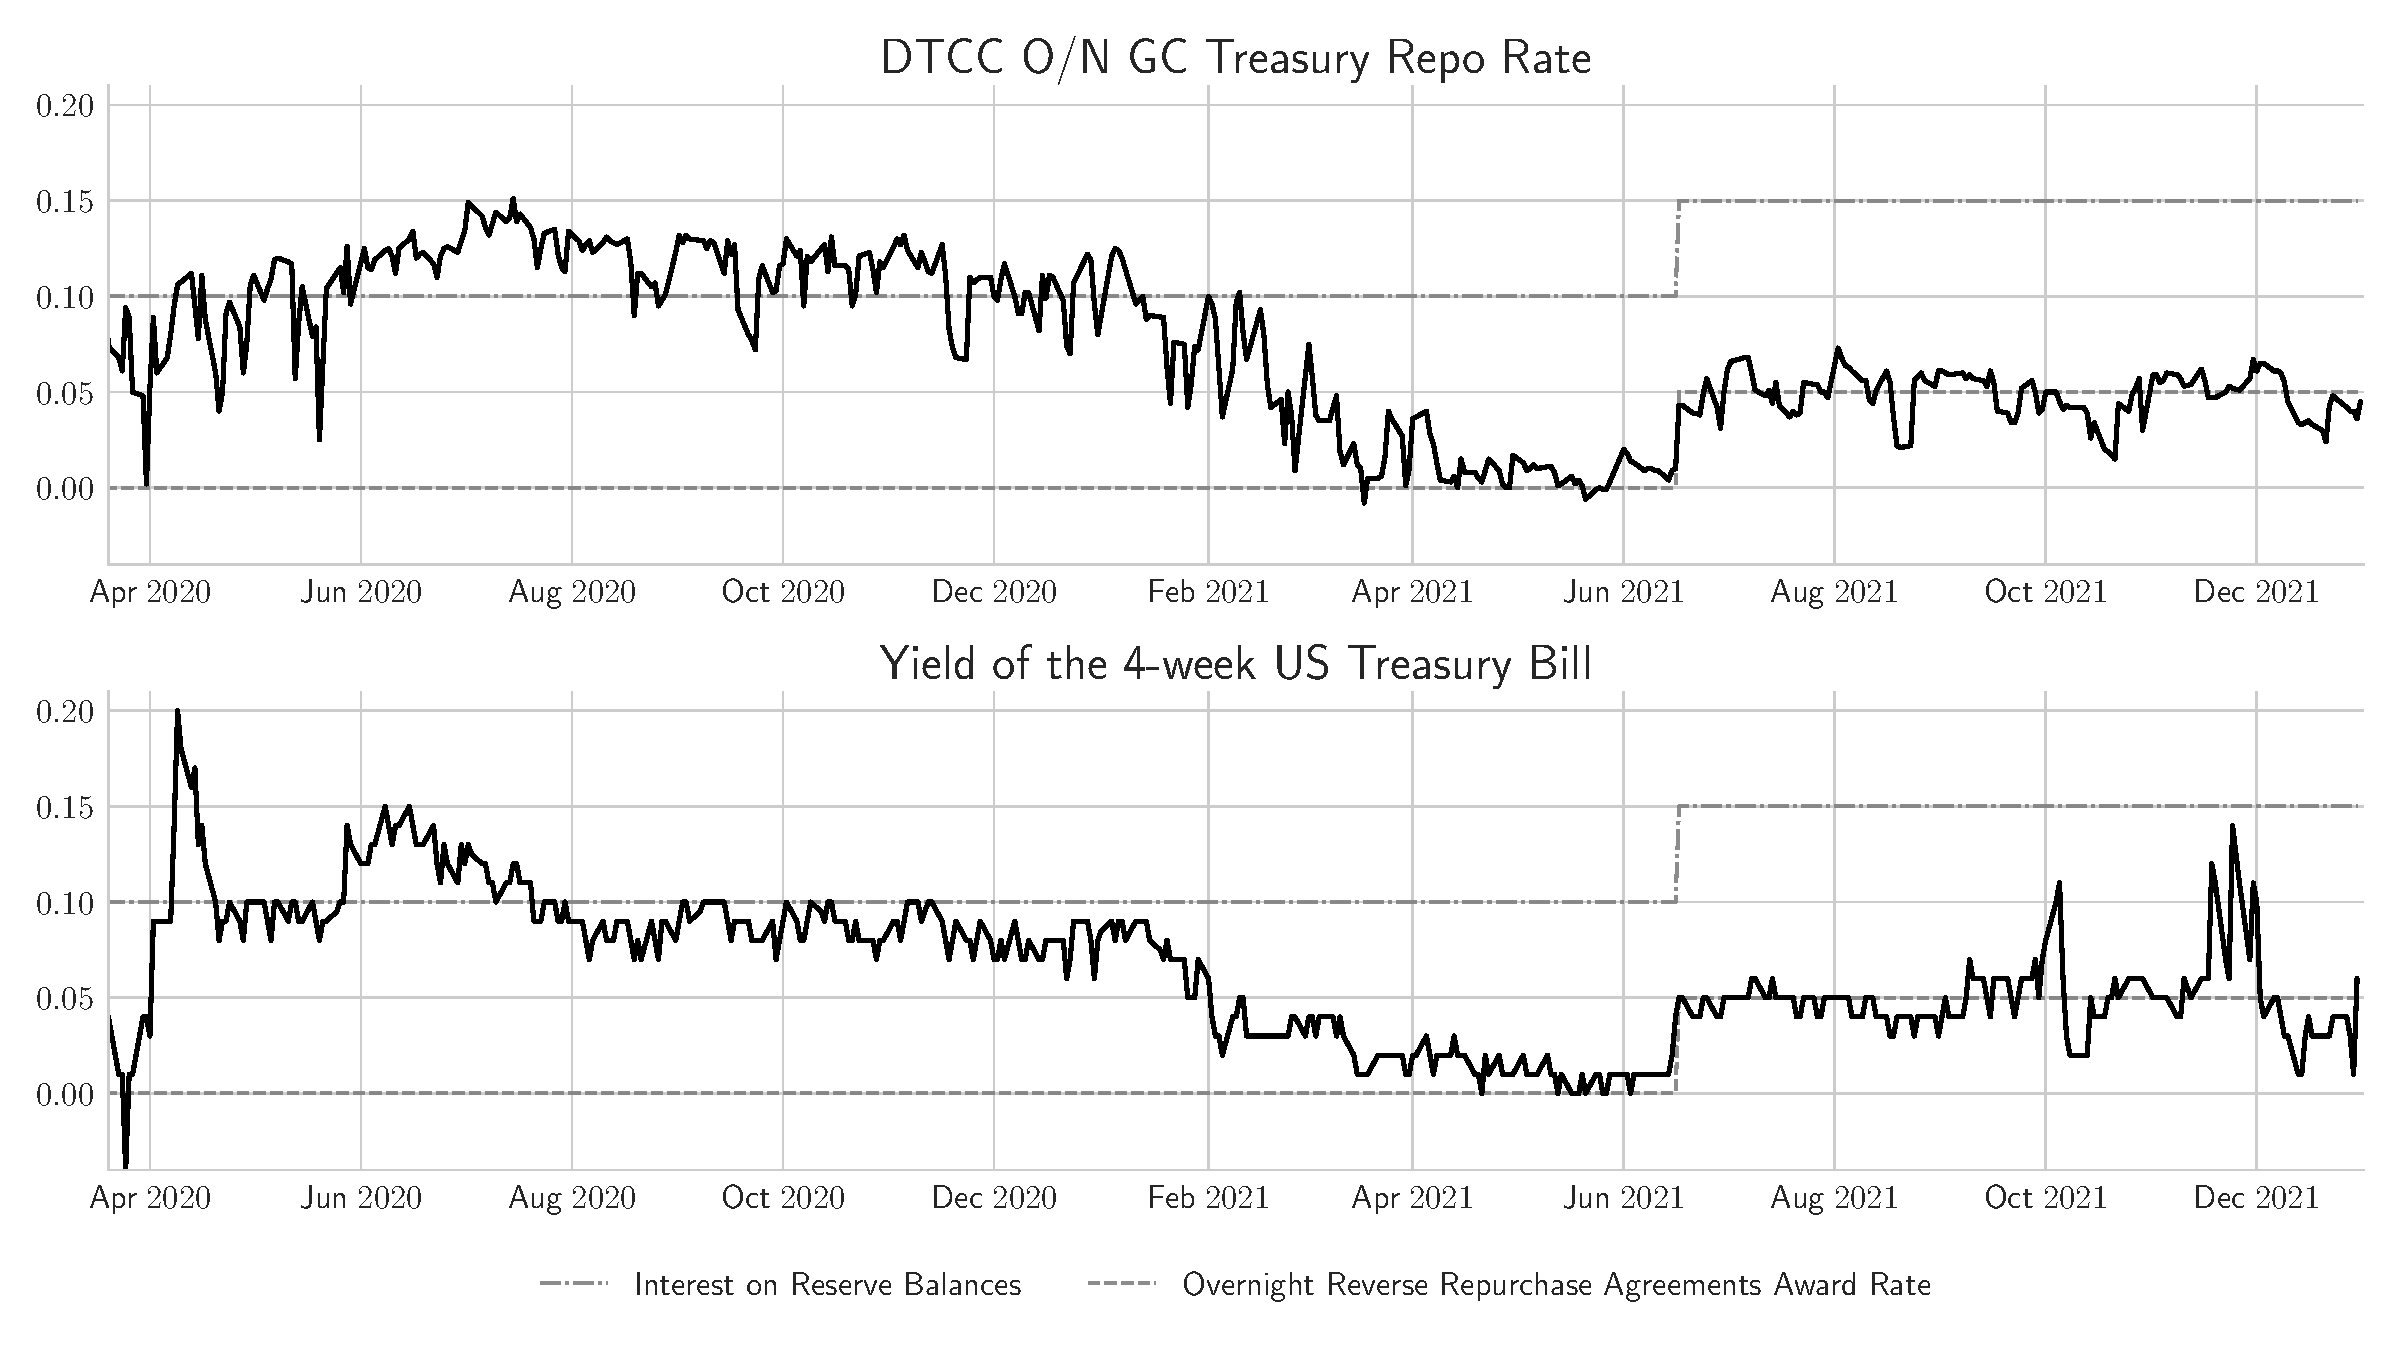
\includegraphics[width=0.99\linewidth]{rates.pdf}
  \end{center}
  \label{fig:rates}
\end{figure}

The supply of Treasury collateral doesn't only come from the debt issuance of the US government, but also from the shadow banking system that creates off-balance sheet collateral on top of the already existing one (see section \ref{sec:mechanics}). It's hard to estimate how much off-balance sheet collateral was created in the last two years, since the start of the pandemic. Nonetheless, by looking at the total received collateral (that is allowed to be re-used) by banks, we can get a broad idea of the dynamics of the shadow banking collateral.

Figure \ref{fig:rrp+coll} shows on the left side the Fed's RRP facility volume, and on the right side the total collateral of Goldman Sachs (on-balance sheet plus off-balance sheet). It is not clear whether there is a casual connection between these time-series, but I argue, that the increase in both is caused by the same underlying condition, which is a scarcity of high-quality collateral. Despite that the plot on the right shows only the collateral of one bank, I found that most of the American G-SIB  banks, except J.P. Morgan, saw the same dramatic increase in received collateral. Surely, fiscal programs that pumped up the Treasury General Account with cash and stuffed primary dealers with Treasuries did increase those bank collateral figures. It has to be noted, though, that at the same time the Treasury deluge was balanced by the Fed's QE4 that withdrew a portion of the new supply of Treasuries from the market. Furthermore, from March 2020 to the end of 2021, the Treasury debt increased 25\%, and if we look at the available collateral of Goldman Sachs, its value, in the same period, increased by 50\%. In short, in 2020-21 we saw a very quickly growing pool of collateral that was driven not only by rising US government debt but also by a rapidly expanding off-balance sheet collateral.

Ultra-low money market rates, all-time high volume of the RRP facility and highly elevated banks' total collateral numbers suggest that the problem lies in the supply-demand misalignment of high-quality collateral.

This section does not prove that scarcity effects exist, but shows how a prolonged QE4 program may be responsible for extremely low money market rates of Treasury securities. The next section takes a 14-year time frame and tries to empirically link the supply factors for Treasury collateral with the Treasury GC repo rate to prove scarcity effects of the Fed's quantitative easing programs.

% Unfortunately, there is not enough quality data to include off-balance sheet collateral creation in this study.

% Figure: RRP and GS collateral
\begin{figure}[htb!]
  \begin{center}
    \caption{RRP, GS Coll}
    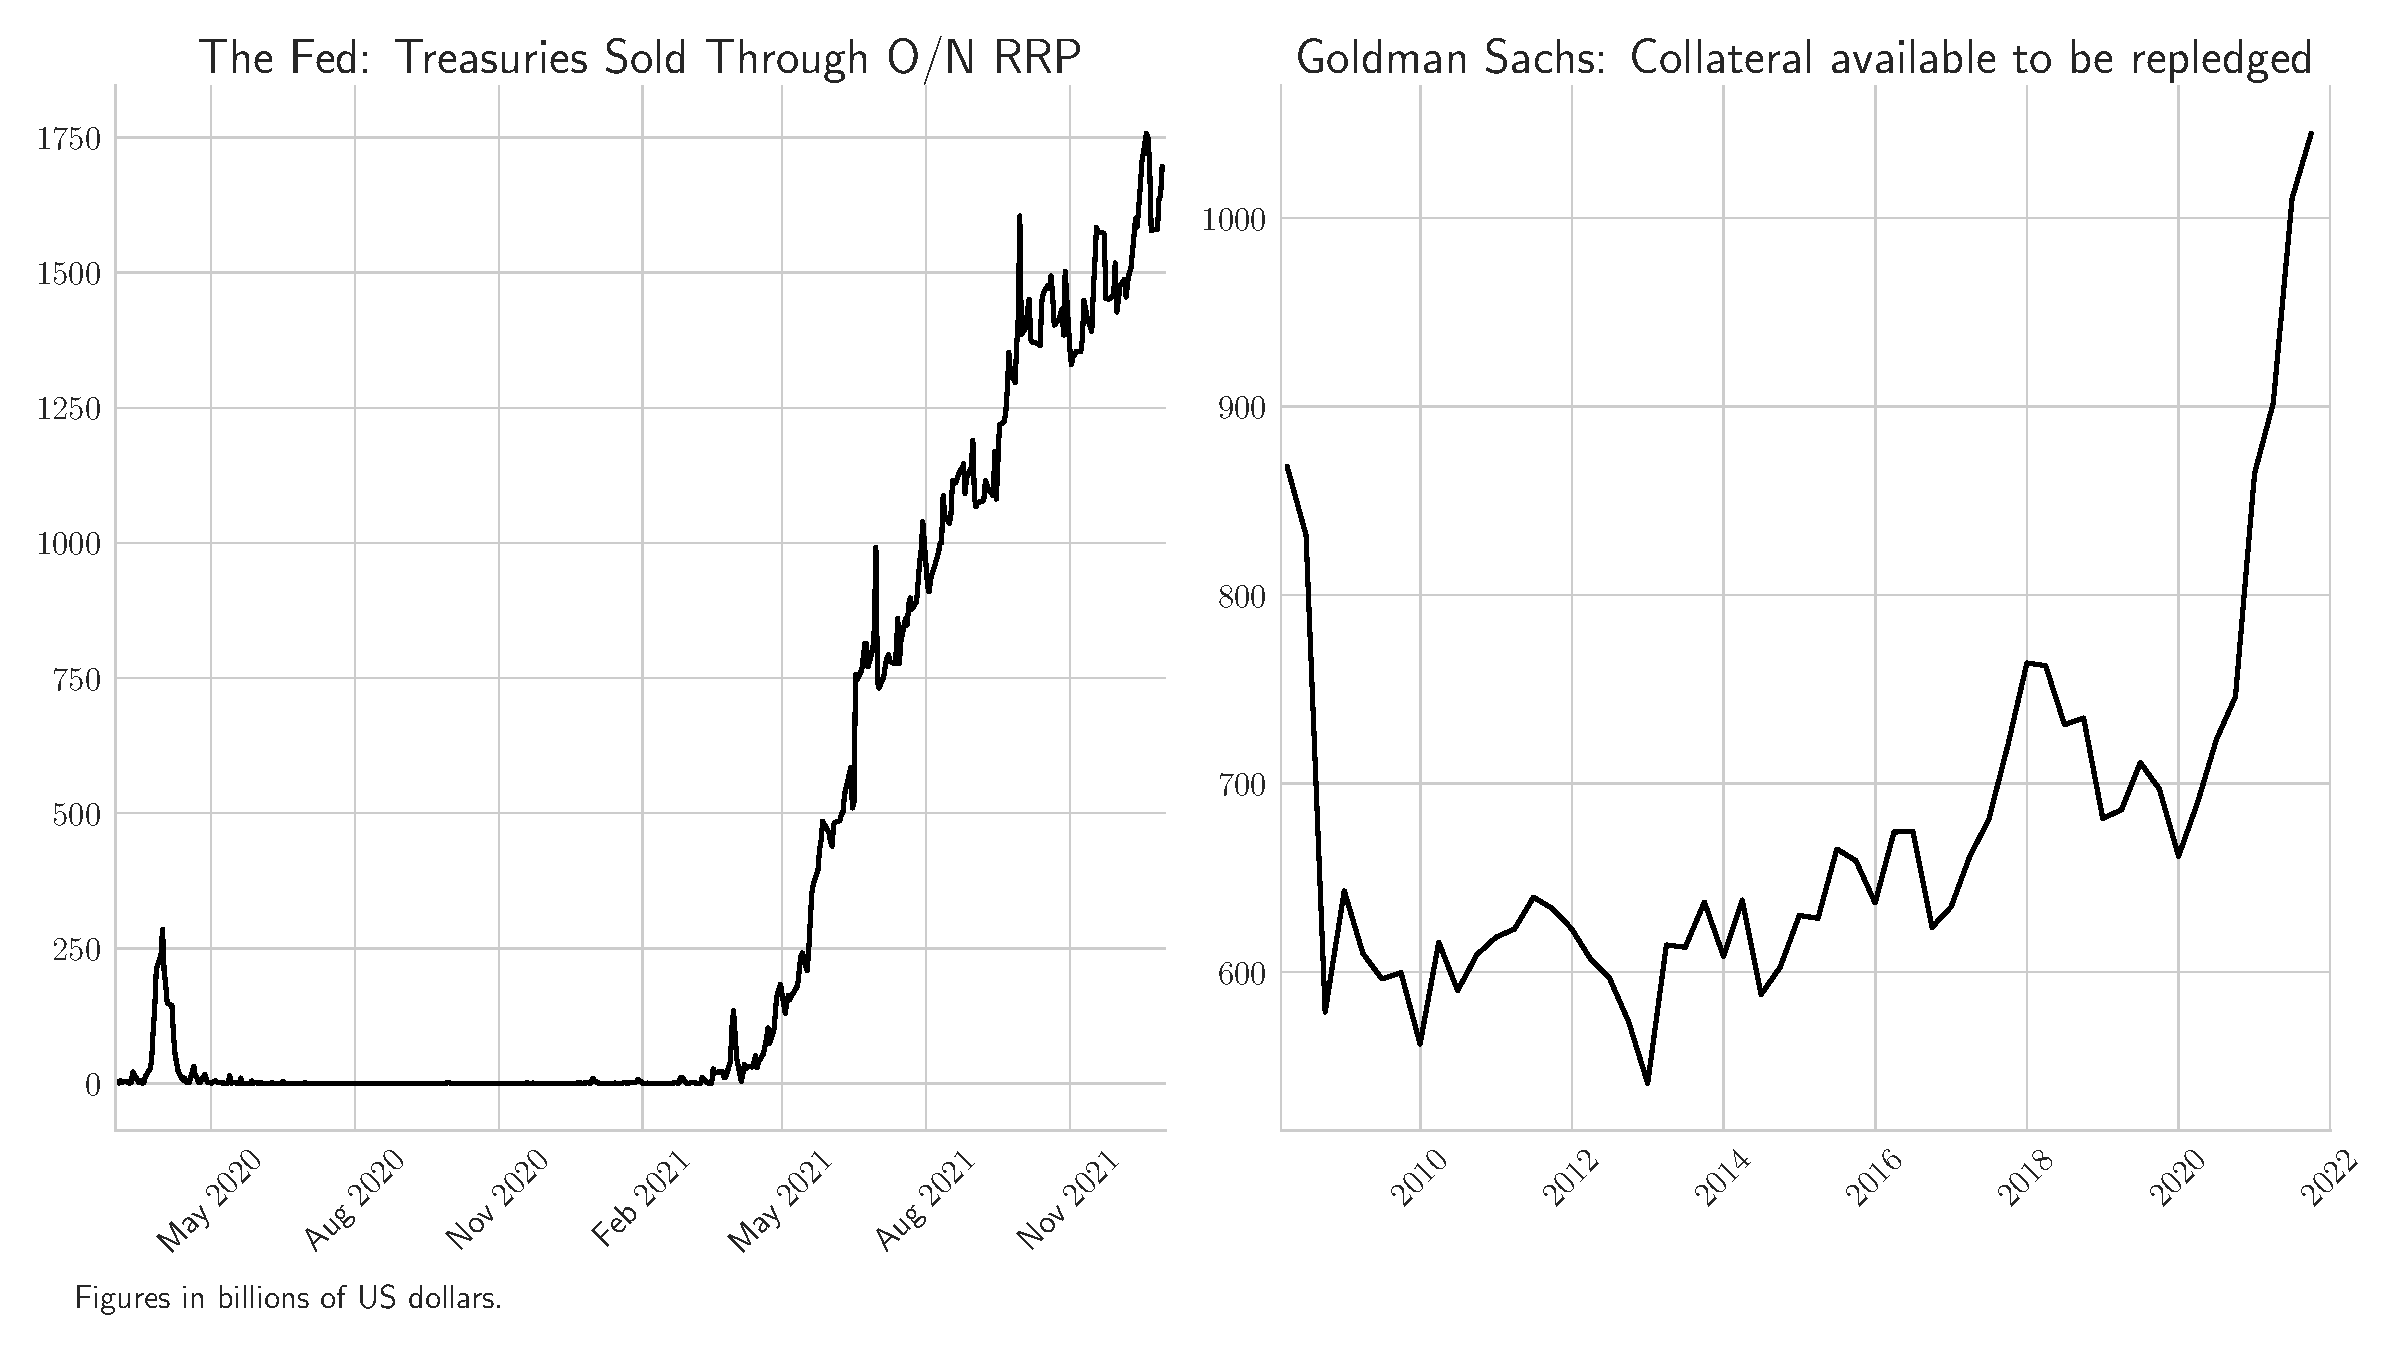
\includegraphics[width=0.99\linewidth]{rrp+coll.pdf}
  \end{center}
  \label{fig:rrp+coll}
\end{figure}

\newpage
 
% ----- EMPIRICAL ----- 
\section{Empirical tests} \label{sec:empirical}

% Data
\subsection{Data} \label{sec:data}

The three main variables that are studied in this research are: the Fed's System Open Market Account (SOMA) Treasury holdings, General Collateral Finance (GCF) Treasury overnight repo rate and the USD collateral spread.

Repo rate data comes from The Depository Trust \& Clearing Corporation (DTCC). The rate is a weighted-average rate of repo contracts that are backed with repo-eligible Treasuries with maturity less than 30 years (CUSIP: 371487AE9). It tracks the average daily interest rate paid for the most-traded GCF Repo contracts for US Treasury securities. DTCC clears a wide variety of repo trades that include bilateral, centrally cleared tri-party and broker-to-broker trades. The rate aggregates information from each of these markets and doesn't specify just one domain of repo contracts.

Collateral spread is the difference between an unsecured and secured money market rate. An unsecured financing normally is more expensive than a secured one, since secured lending (e.g. a repo contract) is safer to the party that lends legal tender money. Over the last 15 years, that have not always been the case, though, as shown in the second plot of figure \ref{fig:vars}. \citet{nyborg2019a} explains what drives collateral spread and why it sometimes turns negative. Here, the collateral spread, for the US market, is defined as the difference between the ICE overnight USD LIBOR rate and the overnight GCF Treasury repo rate. Expressing the repo rate in the form of a collateral spread is important when analyzing dynamics of collateral, and it's impact on money markets.

Scarcity effects should be most visible in the repo rate because engaging in a reverse repo contract is the cheapest way of obtaining collateral securities. This analysis uses one general collateral repo rate, as opposed to special repo rates. The reason for such decision is twofold. First, there haven't been done any studies on scarcity effects that investigate a general collateral (GC) repo rate of Treasury securities on a macro level. Second, data for the rate is easily accessible online. Using a GC rate is also convenient because it removes a necessity to include controls for "specialness" and short selling of a special security. On the other hand, it is hard to include the market microstructure factors when using a general collateral rate, especially with the weekly data frequency that is applied in this study.

To gauge the volume of Treasury securities on the Federal Reserve balance sheet, I use the System Open Market Account Holdings (SOMA) data. SOMA holding are Fed's assets acquired via open market operations. To make the data relevant for this study, I only include the sum of Treasury bills, notes and bonds, and leave out mortgage backed securities and federal agency securities.

Increase in the Fed's SOMA Treasury holdings reduce the supply of government security collateral, however, increase in the Treasury debt outstanding has the opposite effect. I use Debt to Penny daily data of all federal debt outstanding, except debt held by intergovernmental institutions. This time-series is re-sampled to weekly Wednesday levels to match the frequency of the Fed's Treasury holdings.

The recently popular reverse repo standing facility of the Federal Reserve can also alleviate any potential shortage of Treasury collateral, thus I include these figures as well. For a more detailed analysis of the Fed's RRP sale volumes, please see section \ref{sec:shortage}.

To control for other factors that move the repo rate and the collateral spread, I include three other variables, namely the VIX volatility index, 1-month yield on US Treasury bill and a yield curve spread defined as 10-year US Treasury yield less 3-month US Treasury yield. All non-dummy variables are defined in table \ref{table:variables}.

Lastly, there are four categorical variables used to control for changes in the Fed's monetary policy stance. Two of them show when the Fed rises or lowers the fed funds target rates, and the other two indicate dates when the Fed expands or normalizes its balance sheet. The dates can be seen in table \ref{table:dates}, in the appendix section.

% Table: Variables
\begin{sidewaystable}[htbp!] \centering
\caption{Explanation of variables.\\
  All data was accessed and transformed on 10th March 2022.}
{\renewcommand{\arraystretch}{2.2} 
\begin{tabular}{lll}
\toprule
  \textbf{Variable} & \textbf{Definition} & \textbf{Source} \\
\midrule
  TREASURY REPO RATE &  \makecell[l]{GCF (General Collateral Finance) Treasury repo rate\\weighed index composed of GCF repo-eligible CUSIPs:\\U. S. Treasury $<$ 30-year maturity, in bps} & www.dtcc.com\\
\hline
  LIBOR & ICE "Panel Bank" Overnight USD LIBOR rate, in bps & Bloomberg\\
\hline
  COLLATERAL SPREAD & USD ON LIBOR rate minus the Treasury repo rate, in bps & \\
\hline
  UST 1M & Yield on generic 1-month US Treasury bill, in bps & home.treasury.gov\\
\hline
  YIELD CURVE & \makecell[l]{10-year US Treasury note yield  minus 3-month US Treasury\\bill yield, in bps} & home.treasury.gov\\
\hline
  SOMA TREASURIES & \makecell[l]{Fed's Treasury securities at System Open Market\\Account holdings, tril USD} & www.newyorkfed.org\\
\hline
  DEBT & Debt held by the public (debt to penny data), in tril USD & fiscaldata.treasury.gov\\
\hline
  RRP & \makecell[l]{Fed's Overnight Reverse Repurchase Agreements -- Treasury\\securities sold by the Federal Reserve in the temporary\\Open Market Operations, in tril USD} & fred.stlouisfed.org\\
\hline
  VIX & Chicago Board Options Exchange's CBOE Volatility Index & finance.yahoo.com\\
\hline
  PD FAILS & \makecell[l]{Repo fails to receive and fails to deliver, US Treasury\\securities, Primary Dealer Statistics, in tril USD} & www.newyorkfed.org \\
  \bottomrule
\end{tabular}}
% \begin{flushleft}
% \hspace{35pt}\textit{* .}
% \end{flushleft}
\label{table:variables}
\end{sidewaystable}

The time range of the whole data set\footnote{Except primary dealer statistics data that is used in one regression in the appendix.} goes from January 2, 2008, to December 29, 2021. All data has weekly frequency, Wednesday levels. Dollar values are in trillion USD, rate values are in basis points (bps). Table \ref{table:stats} shows descriptive statistics of the data used in regression analysis. All of the data, except the LIBOR rate, comes from free online resources. More details can be found in table \ref{table:variables}.

% Stats
\subsection{Descriptive Statistics} \label{sec:stats}

Figure \ref{fig:vars} shows the evolution of the main variables in the last 11 years. The period of the two years that precede the onset of the 2020 pandemic, was the time of balance sheet normalization. Quantitative tightening started at the end of October 2017 and lasted almost two years until the repo rumble on 17th September 2019. Over that period, the Fed allowed Treasury securities and mortgage-backed securities to roll off their balance sheet. The pace of reducing Treasury holdings was \$12 billion per month, on average. At the same time, the general collateral Treasury repo rate often spiked above the Fed funds upper target and the collateral spread, for almost the whole period, was negative. Interestingly, during times of QE and "taper", when securities weren't systematically bought or sold by the Fed, the collateral spread never stayed negative for so long as it did during the QT.

Table \ref{table:stats} shows basic statistics of the dataset. The average value for the collateral spread, including year 2008, was about 2.9 basis points. If we exclude the whole year 2008 from the sample, the average value changes to -1.5 basis points (median is -0.8). This implies that since 2009, the secured rate for interbank liquidity was lower than the unsecured one. The observation is bizarre, to say the least, since secured lending is much safer than lending that takes place without pledging any collateral.

The average pace of the US debt expansion before the 2020 pandemic was \$760 billion per month. From March 2020 to the end of 2021, the total value of the US debt increased by \$5.3 trillion, which is 30\% of the level recorded in March 2020.

The standing reverse-repo facility was opened for the first time in September 2013. Since that date, until the end of 2017, the average volume of overnight RRP Treasury sales was about \$110 billion. The RRP facility exploded in June 2021, roughly around the time when the RRP award rate increased from 0 bps to 5 bps. Since May 2021, Fed's RRP overnight Treasury sales surged from about \$0.25 trillion to over \$1.6 trillion at the end of the year.

% Figure: Main variables
\begin{figure}[htb!]
  \begin{center}
    \caption{Development of primary variables.}
    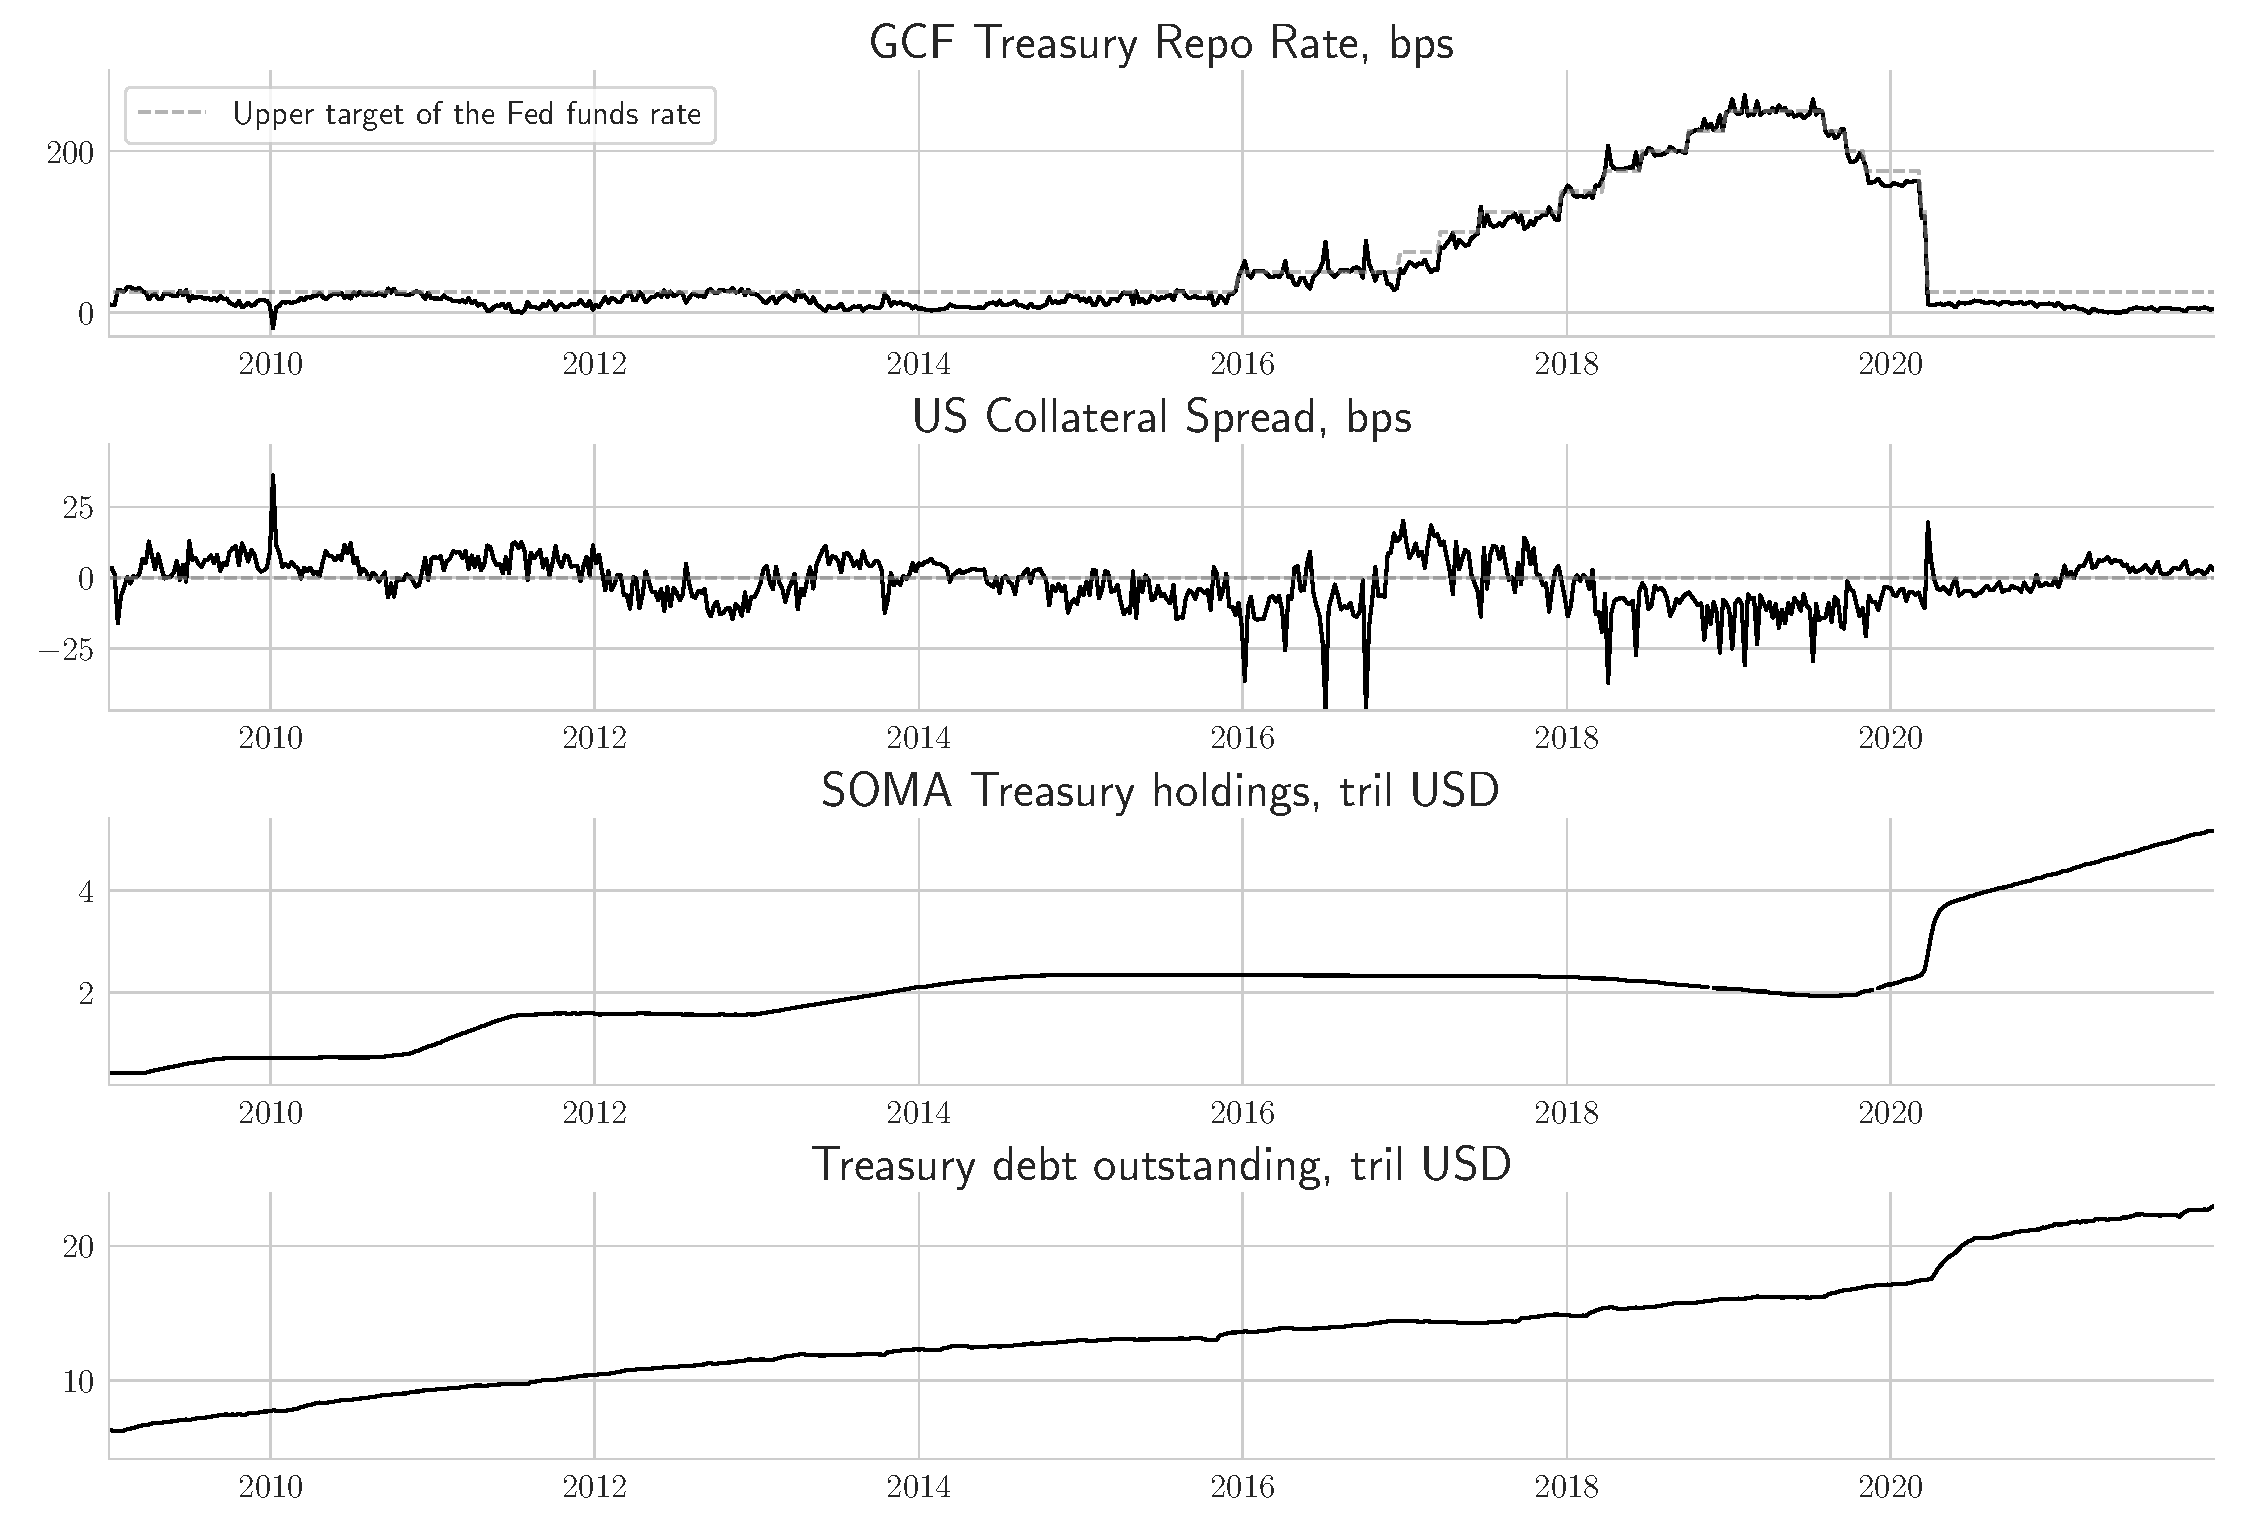
\includegraphics[width=0.99\linewidth]{main_vars.pdf}
  \end{center}
  \label{fig:vars}
\end{figure}

% Table: Statistics
\begin{table}[!h] \centering
\begin{threeparttable}
\caption{Descriptive statistics.}
\begin{tabular}{lrrrrr}
\toprule
{} &    mean &    min &     max &    std &  obs \\
\midrule
GCF Treasury O/N repo rate (bps) &   64.00 & -19.30 &  418.40 &  82.63 &  732 \\
Collateral spread, USD (bps) &    2.89 & -47.11 &  495.28 &  29.63 &  731 \\
O/N USD LIBOR rate (bps) &   66.97 &   5.46 &  509.38 &  87.47 &  731 \\
1-month UST yield (bps) &   51.52 &   0.00 &  337.00 &  77.08 &  732 \\
10-year less 3-month UST yield (bps) &  183.24 & -49.00 &  380.00 &  96.53 &  732 \\
Treasury SOMA holdings (tril USD) &    2.04 &   0.43 &    5.17 &   1.12 &  729 \\
Treasury debt outstanding (tril USD) &   13.00 &   5.10 &   23.03 &   4.47 &  732 \\
Fed's RRP standing facility volume (tril USD) &    0.09 &   0.00 &    1.70 &   0.25 &  732 \\
VIX volatility index &   20.15 &   9.19 &   80.86 &   9.76 &  732 \\
% Treasury security repo fails (all fails) &    0.19 &   0.06 &    0.89 &   0.11 &  457 \\
\bottomrule
\end{tabular}
Observations from January 2, 2008 to January 5, 2022. The data above is not transformed, however, regressions in the following section apply first-differencing.
 % (except the last variable which data starts from April 3, 2013)
\label{table:stats}
\end{threeparttable}
\end{table}

% Base model
\subsection{Base regression specification} \label{sec:base}

The main objective of this paper is to determine whether the Fed's Treasury buying programs make Treasury securities significantly more scarce in the market. To see that, I test a casual connection between Treasury security supply factors and the GCF Treasury repo rate with a simple linear regression. All data put into regressions is in a first difference form in order to remove trends and make time-series stationary.

There are two sets of OLS regressions with two different dependent variables. My basic regression specification involves the general collateral repo rate as the dependent variable and a set of independent variables that reflect supply and demand factors for collateral. The following is the base regression equation

\begin{equation} \label{eq:1}
  \begin{gathered}
  \Delta \textit{Treasury Repo Rate} = \beta_0 + \beta_1 \Delta \textit{SOMA Treasury}_t + \beta_2 \Delta \textit{Debt}_t \\ + \beta_3 \Delta \textit{RRP}_t  + \beta_4 \Delta \textit{UST 1M}_t + \gamma \textit{Controls}_{i,t} + \epsilon_{t}.
  \end{gathered}
\end{equation}

$\Delta$ SOMA Treasury and $\Delta$ Debt variables are supply factors of the underlying collateral. The former shows to what extent the Fed draws Treasury securities out of the market, and the latter variable represents the pace of the US government collateral provision to the market.

The Fed's RRP standing facility sales are initiated by agents that seek to lend reserves to the central bank, and in return want to receive collateral. Therefore, Treasury sales that go through the RRP facility are a demand factor for collateral. The Fed's reserve-repo rate sets the floor for Treasury bill rates. A high volume of those sales indicates, that without such facility, short term rates could dip below the central bank's range of the policy rate. The thinking that goes behind the connection between the RRP and the demand for Treasury collateral is presented in section \ref{sec:shortage}.
The value RRP facility transactions alone cannot capture all the demand that exists for liquid Treasury securities. It is so because only eligible parties can access central bank facilities, and the price of those reverse-repo contracts is set only by the Fed. In order to account for demand for Treasury securities in the wider market, I use the $\Delta$ UST 1M variable, which is a yield on a generic one-month Treasury bill. It has been documented that a repo rate moves together with the yield of its collateral security traded in the cash market (\citep{bartolini2011}, \citep{nyborg2019a}).

To capture the effect of other determinants of the repo rate, I incorporate two more macro variables, as well as four categorical variables that control for changes in monetary policy. Those additional macro variables are the VIX stock volatility index and the UST yield curve.

% vix controls for ..., and tield curve controls for ...

% Problem with the unsecured rate
\subsection{Problem with the unsecured rate} \label{sec:unsecured}

Evidence from the European repo market shows that special repo rates are driven mostly by search costs of a specific collateral (\citep{schaffner2019}). Meaning that, special repo markets are primarily markets for collateral. On the other hand, general collateral repo markets should be driven more by the demand for cash liquidity, as those contracts identify the collateral only after all other terms of the trade are agreed. If the received security, that acts as collateral, is not strictly specified, we should assume that those repos are used to secure short-term funding just as in the unsecured market. Thus, it is essential to account for demand for cash liquidity factor, that is not associated with collateral when examining repo rates.

The unsecured rate, which in this case is the US dollar O/N LIBOR rate, is an important component that indicates the price of dollar liquidity. However, simply including it in the regression as a right-hand side variable may not be the best solution due to a potential reverse causality problem.

Since the Global Financial Crisis, activity in the unsecured money market segment have been declining. In 2003, the split of the total lending turnover was roughly equal, but by 2015 the size of the unsecured market was only one-tenth of the total \citet{fiore2018}. Much bigger and liquid secured markets imply that a demand for funds should be more precisely captured in general collateral repo rates. In other words, it may be that the secured rate sets the price of overnight money, which then feeds into the rate of unsecured funds, and not the other way around.

In this study, I use an overnight USD LIBOR rate as an unsecured rate, which further complicates this problem. The rate is set not by the market, but by a panel of 15 large banks. Using the fed funds isn't a good substitute either because of its market structure. There are two sets of major players in the fed funds market: Federal Home Loan Banks and foreign banks with branches in New York. That makes it a rather shallow market with a very low volatility compared to the repo market. For example, since September 1st, 2021 until December 30th of the same year the effective fed funds rate was 8 basis points every single day. Volatility is almost non-existent. Sudden spikes in the fed funds rate sometimes happen, but only when the intraday liquidity in the repo market dries up. In that case, dealers keep daylight overdrafts at the clearing bank (Bank of New York) and those intraday loans become overnight GC repo. In order to settle its own overdrafts with the Fed, the clearing bank borrows then in the O/N fed funds market, and the effective fed funds rate picks up some volatility (\citep{gmn22}.

The peculiarities of the fed funds market make the O/N USD LIBOR rate a better choice when it comes to the price of an overnight dollar, but having that rate as a regressor is undesirable. What can be done is transforming the dependent variable.

\begin{equation} \label{eq:2}
  \begin{gathered}
    \Delta \textit{Collateral Spread} = \beta_0 + \beta_1 \Delta \textit{SOMA Treasury}_t + \beta_2 \Delta \textit{Debt}_t \\ + \beta_3 \Delta \textit{RRP}_t + \beta_4 \Delta \textit{LIBOR}_t + \beta_5 \Delta \textit{UST 1M}_t + \gamma \textit{Controls}_{i,t} + \epsilon_{t}
  \end{gathered}
\end{equation}

A simple substitution of collateral spread for the repo rate removes the problem. The collateral spread, being the difference between the unsecured and secured rate, should eliminate most of the variability that is caused by the demand for funds, as both rates respond to that occasion in the same direction. For this reason, the second specification sets the collateral spread as the dependent variable and puts the O/N USD LIBOR rate on the right-hand side of the equation to control for any tightness in the unsecured market. Conditions in the unsecured interbank market for liquidity still affect the collateral spread \citet{nyborg2019a}, so the unsecured rate is included as a dependent variable.

Other known determinants of the collateral spread are liquidity, volatility, haircut of the underlying security, and risk-aversion. Regarding attributes of the underlying security in the cash market, it is not clear which security in particular should be analyzed, as my repo rate covers a wide variety of Treasuries. For instance, on-the-run Treasury bills are much more liquid than off-the-run Treasury bonds. Because of that reason, I don't use any liquidity metric and I proxy the overall volatility in the markets as well as risk-aversion with the VIX index. Haircuts are not taken into account, as all Treasury securities are deemed to have the same level of safety.

There is also one Treasury supply factor that should be included in my regressions but isn't due to the unavailability of a high-frequency metric for that factor. It is a variable that represents the re-use rate of collateral in the monetary system. The more often source collateral is re-used in the system, the more collateral can be utilized. Rehypothecated collateral acts like a synthetic Treasury derivative, so more rehypothecation would mean more demand for that collateral  Some banks put the amount of received  collateral that is allowed to be repledged in their quarterly reports. Unfortunately, the size of that data is too small to be meaningful given the time frame of this study.

% Results
\subsection{Results} \label{sec:results}

The two sets of regressions, which results are shown in the tables below, confirm the hypothesis that the Fed's purchases of Treasuries put a downward pressure on the GCF Treasury repo rate, and so an upward pressure on the US collateral spread. A high and statistically significant coefficient for the SOMA Treasury holdings variable in each regression specification suggest that the scarcity effects from quantitative easing programs are real.

Table \ref{table:reg1} shows how supply factors of US Treasury collateral affect the general collateral Treasury repo rate. The coefficient next to "SOMA TREASURY" variable in the second column of the table (-45.5) implies that a \$1 trillion Treasury purchase by the Fed causes the repo rate to decline, on average, by 45.5 basis points, with all other determinants held constant. The magnitude of the effect in this paper is much smaller than in \citet{damico2014}, however, that study is much different as it looks on special repo rates as opposed to the general collateral repo rate.

\citet{damico2014} find that a \$1 billion purchase of off-the-run US Treasury securities by the Fed lowers a SC repo rate by 0.2-0.33 basis points. This implies that the impact of QE on special repo rates is about 4 times bigger impact than on general collateral Treasury repo rate. The result aligns well with findings in the literature on special repo rates. Special repo rates react more to changes in collateral supply, but general collateral rates that are backed with a specific type of security are still prone to changes in the fundamentals of collateral. It has to be noted, though, that, naturally, supply of a specific (i.e. "special") security is lower than supply of the GCF Treasury basket aggregate. Also, \citet{damico2014} apply a panel regression with a range of SC rates over a 4-year time frame and a daily frequency of the data, which is a completely different set up.

Three regressions are included in table \ref{table:reg1}, where the dependent variable is the GCF Treasury repo rate. The first column looks only at the value of US Treasuries on the Fed's balance sheet and the total value of US Treasury debt outstanding. The most important supply factors. \citet{damico2014} and \citet{arrata2018} merge two of these values into one variable, that is, a ratio of the former to the latter. Here, I put those variables separately to understand the relative magnitude of both. As illustrated in the table, taking high-quality Treasury collateral out of the market affects the repo rate more than the US Department of Treasury provision of these collateral securities. The second column adds other important factors that move the repo rate. All of them are statistically significant. Including those factors addresses the omitted variable bias, as both coefficients of the SOMA variable and the debt variable are much smaller after the addition of those controls in the model.

% Regression table 1: GCF repo rate
\begin{table}[!htbp] \centering
\caption{Regression --- GCF Treasury repo rate and the supply of Treasury securities}
\begin{tabular}{@{\extracolsep{5pt}}lccc}
\\[-1.8ex]\hline
\hline \\[-1.8ex]
& \multicolumn{3}{c}{\textit{Dependent variable: General Collateral Treasury Repo Rate}} \
\cr \cline{3-4}
  \\[-1.8ex] & (1) & (2) & (3) \\
\hline \\[-1.8ex]
 Intercept & -0.818$^{}$ & -0.265$^{}$ & -0.353$^{}$ \\
  & (0.568) & (0.295) & (0.285) \\
 SOMA TREASURY & -91.651$^{**}$ & -45.549$^{***}$ & -44.646$^{**}$ \\
  & (45.276) & (17.261) & (17.389) \\
 DEBT & 33.710$^{***}$ & 23.180$^{**}$ & 23.794$^{**}$ \\
  & (12.068) & (10.366) & (10.587) \\
 RRP & & 30.961$^{**}$ & 31.462$^{**}$ \\
  & & (13.603) & (13.843) \\
 UST 1M & & 0.630$^{***}$ & 0.648$^{***}$ \\
  & & (0.123) & (0.121) \\
 YIELD CURVE & & -0.127$^{**}$ & -0.114$^{*}$ \\
  & & (0.063) & (0.068) \\
 C(RATE DOWN) & & -36.442$^{***}$ & -36.194$^{***}$ \\
  & & (7.825) & (7.793) \\
 C(RATE UP) & & 19.735$^{***}$ & 19.476$^{***}$ \\
  & & (1.758) & (1.870) \\
 VIX & & & 0.143$^{}$ \\
  & & & (0.154) \\
 C(FED EASING) & & & 5.917$^{*}$ \\
  & & & (3.026) \\
 C(FED TIGHTENING) & & & -2.004$^{}$ \\
  & & & (1.373) \\
\hline \\[-1.8ex]
 Observations & 726 & 726 & 726 \\
 Adjusted $R^2$ & 0.020 & 0.504 & 0.506 \\
\hline
\hline \\[-1.8ex]
  & \multicolumn{3}{r}{$^{*}$p$<$0.1; $^{**}$p$<$0.05; $^{***}$p$<$0.01} \\[8pt]
\end{tabular}
\begin{flushleft}
  \textit{Notes: All variables, except categorical "C" ones, are in first-difference form. Standard errors are heteroscedasticity and autocorrelation robust (HAC) using 5 lags and without small sample correction (in parentheses). All variables are defined in table \ref{table:variables}.}
\end{flushleft}
\label{table:reg1}
\end{table}

I exclude a possibility of reverse causality of the dependent variable and the main regressor, which is the Fed's Treasury holdings variable. The reason for this is the fact that the Fed alleviated the scarcity effect of bond purchases only once. It was done through a regulatory instrument, which was a Supplementary Leverage Ratio (SLR) relief to banks in March 2020. A temporary exclusion of Treasuries and central bank reserves definitely freed up some balance sheet space of banks and allowed banks to hold more Treasuries, but it had not much to do with Treasury purchases under QE programs. Moreover, the SLR relief probably targeted the increased cost of holding a high amount of reserves in the banking system rather than Treasuries.

Column 3 adds the VIX index and dummy variables that represent the dates when the Fed clearly took action in regard to the size of their balance sheet. Initiating or expanding quantitative easing contributed to rising repo rate, and doing the opposite, seemingly, decreased the dependent variable. However, the coefficient of the last variable, which is a dummy for tightening balance sheet dates, is not statistically significant. The coefficient of the implied volatility index is also not significant.

There are two reasons why adding QT dates variable to the regression generates a high p-value. First, quantitative tightening is a very careful and gradual process. This is contrary to announcements of QE programs, which are often sudden and act as a response to an economic or monetary crisis. Second, termination dates of some liquidity providing programs sometimes overlap with other fully-fledged security purchase programs that are in the still in progress. For instance, in June 2020 the Fed stopped a liquidity support to the repo market, which had begun as an effect of a stress in that market on 17th September 2019. However, at the same time, it was still buying securities on a massive scale under the QE4 program. These quantitative easing/tightening dates can be found in table \ref{table:fed} in the appendix.

Notably, the reverse-repo standing facility had a substantial impact on the direction of the repo rate. The effect is large and significant. A positive coefficient suggests that the more Treasuries are borrowed from the Fed (through a reverse repo contract), the more collateral can be utilized by money market participants. This, in turn, makes the desired collateral more plentiful, which pushes the repo rate up.

Table \ref{table:reg2} presents the results of running the second model specification. It does not differ from the former one in a great extent. The only major difference is the dependent variable, which in this case in the US collateral spread. As described in section \ref{sec:unsecured}, this transformation of the dependent variable allows including the unsecured rate in the model.

The interpretation of results in table \ref{table:reg2} is the opposite to those that are in the table \ref{table:reg1}. For example, the coefficient of the variable that represents the size of SOMA holdings in the column 3, which is 41.8, suggests that a \$1 trillion increase in Treasury securities on the Fed's balance sheet, causes the collateral spread to widen by about 42 basis points. Considering, that the model controls for the LIBOR rate, we can say that this effect is caused solely by an increasing repo rate. As the collateral spreads widens and the unsecured rate stays constant, the repo rate decreases. Hence, an opposite interpretation.

% Regression table 2: Collateral spread
\begin{table}[!htbp] \centering
\caption{Regrression --- Measuring scarcity effects with collateral spread}
\begin{tabular}{@{\extracolsep{5pt}}lcccc}
\\[-1.8ex]\hline
\hline \\[-1.8ex]
& \multicolumn{4}{c}{\textit{Dependent variable: Collateral Spread}} \
\cr \cline{4-5}
\\[-1.8ex] & (1) & (2) & (3) & (4) \\
\hline \\[-1.8ex]
 Intercept & 0.933$^{}$ & 0.131$^{}$ & 0.256$^{}$ & 0.341$^{}$ \\
  & (0.636) & (0.563) & (0.293) & (0.285) \\
 SOMA TREASURY & 25.869$^{}$ & -12.750$^{}$ & 41.788$^{**}$ & 41.351$^{**}$ \\
  & (22.988) & (30.442) & (17.358) & (17.268) \\
 DEBT & -46.641$^{**}$ & -32.801$^{**}$ & -23.801$^{**}$ & -24.302$^{**}$ \\
  & (19.162) & (16.331) & (10.121) & (10.356) \\
 RRP & & -30.076$^{*}$ & -30.904$^{**}$ & -31.345$^{**}$ \\
  & & (15.854) & (13.664) & (13.866) \\
 UST 1M & & -0.592$^{***}$ & -0.627$^{***}$ & -0.643$^{***}$ \\
  & & (0.198) & (0.118) & (0.117) \\
 YIELD CURVE & & 0.218$^{**}$ & 0.133$^{**}$ & 0.121$^{*}$ \\
  & & (0.090) & (0.059) & (0.064) \\
 C(RATE DOWN) & & 26.161$^{}$ & 35.779$^{***}$ & 35.562$^{***}$ \\
  & & (21.372) & (7.706) & (7.742) \\
 C(RATE UP) & & 3.885$^{**}$ & -18.211$^{***}$ & -18.060$^{***}$ \\
  & & (1.872) & (2.000) & (2.062) \\
 LIBOR & & & 0.935$^{***}$ & 0.938$^{***}$ \\
  & & & (0.044) & (0.043) \\
 VIX & & & & -0.118$^{}$ \\
  & & & & (0.153) \\
 C(FED EASING) & & & & -5.902$^{*}$ \\
  & & & & (3.067) \\
 C(FED TIGHTENING) & & & & 1.974$^{}$ \\
  & & & & (1.396) \\
\hline \\[-1.8ex]
 Observations & 726 & 726 & 726 & 726 \\
 Adjusted $R^2$ & 0.007 & 0.200 & 0.770 & 0.771 \\
\hline
\hline \\[-1.8ex]
  & \multicolumn{4}{r}{$^{*}$p$<$0.1; $^{**}$p$<$0.05; $^{***}$p$<$0.01} \\[8pt]
\end{tabular}
\begin{flushleft}
\vspace{-5pt}
  \textit{Notes: Collateral spread is defined as the difference between USD ON LIBOR rate and ON GCF Treasury repo rate. All variables, except categorical "C" ones, are in first-difference form. Standard errors are heteroscedasticity and autocorrelation robust (HAC) using 5 lags and without small sample correction (in parentheses). All variables are defined in table \ref{table:variables}.}
\end{flushleft}
\label{table:reg:2}
\end{table}

Analyzing scarcity effects in relative terms of a collateral spread, and at the same time controlling for the price of liquidity in the unsecured market, allows to isolate and analyze the collateral-side of a repo contract. This method extracts the portion of a change in a repo rate that is associated only with market conditions of underlying securities. The results are, however, roughly the same for both specifications.

There are a few other repo and collateral spread drivers that are not included in this study. For example, haircut of the underlying security is not included because of the class of these assets (highest-quality) and the unavailability of the data. A liquidity metric of an underlying collateral is also not included because there is no metric that aggregates and provides information about the liquidity status of all Treasury securities\footnote{For instance, on-the run Treasuries are more liquid than off-the-run Treasuries. The same goes for securities with different maturities. T-bills are more liquid than T-bonds.}. I have tried adding other regressors (that controlled for liquidity, volatility, regulatory changes) and were plausible to considerably affect the final result, but none of those variables came out to be statistically significant (see table \ref{table:reg3} in the appendix).

Since September 2019 to the end of 2021, the Fed has purchased over \$2.5 trillion of Treasury securities from the secondary market. According to the results from table \ref{table:reg1} (column 2), this expansion of the central bank's balance sheet is associated with about 113 bps decrease in the repo rate over the whole period. At the same time, the US Treasury Department, through its fiscal stimulus programs, was supplying Treasury securities to the market. Taking two effects into account, the supply factors contributed to about a 56 basis point decrease of the repo rate. There are also demand factors and other drivers of the GC Treasury repo rate that were included in this study. Nonetheless, I refrain from delving too much into interpretation of control variables as effect sizes of those additional variables very rarely have a casual interpretation \citet{hunermund2020}.

All regressions use Newey–West standard errors. The number of lags is equal to the closes integer of the fourth root of the number of observations (726), which is 5. Each variable, except categorical variables, is in the fist-difference form ($X_t-X_{t-1}$).

\newpage %

% ----- CONCLUSIONS ----- 
\section{Conclusions} \label{sec:conclusion} 

% effects of policy normalization 
% \lipsum[1-8]

% ----- APPENDIX (OPTIONAL) ----- 
\newpage

% \appendix
% \noappendicestocpagenum
%\addappheadtotoc
%\appendixpage

% \begin{appendix}
%   \section{A}
% \end{appendix}

\begin{appendices}
% \section{Tables}

% Table: Fed Dates
\begin{table}[!h] \centering
\begin{threeparttable}
\caption{Fed Dates.}
\begin{tabular}{lll}
\toprule
Date & Variable & Event \\
\midrule
25 Nov 2008 & FED EASING & Announcement of QE1 \\
16 Mar 2009 & FED EASING & QE1 Expanded \\
31 Mar 2010 & FED TIGHTENING & QE1 Terminated \\
10 Aug 2010 & FED EASING & QE1 Rollover \\
3 Nov 2010 & FED EASING & Announcement of QE2 \\
21 Sep 2011 & FED EASING & Announcement of Operation Twist \\
20 Jun 2012 & FED EASING & Operation Twist Extended \\
13 Sep 2012 & FED EASING & Announcement and initiation of QE3 \\
12 Dec 2012 & FED EASING & QE3 Expanded \\
31 Dec 2012 & FED TIGHTENING & Operation Twist Terminated \\
18 Dec 2013 & FED TIGHTENING & Start of the QE3 taper \\
29 Oct 2014 & FED TIGHTENING & QE3 Terminated \\
1 Nov 2017 & FED TIGHTENING & QT has begun \\
20 Mar 2019 & FED EASING & The Fed slows down the reduction of its Treasury holdings \\
18 Sep 2019 & FED EASING & Overnight lending repo facility opened \\
15 Mar 2020 & FED EASING & Announcement of QE4 \\
11 Jun 2020 & FED TIGHTENING & The Fed tightness operations in the repo market \\
\bottomrule
\end{tabular}
Observations from January 2, 2008 to January 5, 2022 (except the last variable which data starts from April 3, 2013). The data above is not transformed, however, regressions in the following section apply first-differencing.
\label{table:fed}
\end{threeparttable}
\end{table}

% Regression table 3: Collateral spread, additional variables NEW
\begin{table}[!htbp] \centering
\caption{Regression -- Adding other plausible explanatory variables to the collateral spread specification.}
\vspace{-10pt}
\begin{flushleft}
Variable "UST 3M BID-ASK" is the bid-ask spread of a generic 3-month Treasury bill yield. Variable "UST 3M 10W VOL" is the 10-week realized volatility of a generic 3-month Treasury bill yield. The first column regression uses a smaller data sample that starts April 3, 2013. All newly added variables are not statistically significant (p-values exceed as much as 0.3). Condition number of the third column regression is large which indicates strong multicollinearity.
\end{flushleft}
\begin{tabular}{@{\extracolsep{5pt}}lccc}
\\[-1.8ex]\hline
\hline \\[-1.8ex]
& \multicolumn{3}{c}{\textit{Dependent variable: US Collateral Spread}} \
\cr \cline{3-4}
\\[-1.8ex] & (1) & (2) & (3) \\
\hline \\[-1.8ex]
 Intercept & 0.411$^{*}$ & 0.358$^{}$ & 0.253$^{}$ \\
  & (0.237) & (0.284) & (0.294) \\
 SOMA TREASURY & 28.773$^{}$ & 21.443$^{}$ & 41.205$^{**}$ \\
  & (20.417) & (28.856) & (17.177) \\
 DEBT & -21.732$^{***}$ & -19.209$^{**}$ & -23.466$^{**}$ \\
  & (6.063) & (9.457) & (10.184) \\
 RRP & -27.035$^{**}$ & -30.481$^{**}$ & -31.166$^{**}$ \\
  & (13.337) & (13.516) & (13.612) \\
 UST 1M & 0.013$^{}$ & -0.581$^{***}$ & -0.626$^{***}$ \\
  & (0.117) & (0.154) & (0.119) \\
 LIBOR & 0.109$^{}$ & 0.951$^{***}$ & 0.937$^{***}$ \\
  & (0.276) & (0.035) & (0.043) \\
 YIELD CURVE & 0.178$^{***}$ & 0.153$^{***}$ & 0.133$^{**}$ \\
  & (0.048) & (0.055) & (0.059) \\
 C(RATE DOWN) & 6.631$^{}$ & 36.885$^{***}$ & 35.694$^{***}$ \\
  & (9.963) & (8.863) & (7.720) \\
 C(RATE UP) & -2.429$^{}$ & -19.216$^{***}$ & -18.174$^{***}$ \\
  & (6.177) & (1.903) & (1.983) \\
 PD FAILS & -0.791$^{}$ & & \\
  & (2.826) & & \\
 UST3M 10W VOL & & 0.480$^{}$ & \\
  & & (0.490) & \\
 UST3M BIDASK & & & 0.004$^{}$ \\
  & & & (0.006) \\
\hline \\[-1.8ex]
 Observations & 452 & 716 & 726 \\
 Adjusted $R^2$ & 0.096 & 0.800 & 0.770 \\
\hline
\hline \\[-1.8ex]
 & \multicolumn{3}{r}{$^{*}$p$<$0.1; $^{**}$p$<$0.05; $^{***}$p$<$0.01} \\
\end{tabular}
\begin{flushleft}
\vspace{-5pt}
  \textit{Notes: Collateral spread is defined as the difference between USD ON LIBOR rate and ON GCF Treasury repo rate. All variables, except categorical "C" ones, are in first-difference form. Standard errors are heteroscedasticity and autocorrelation robust (HAC) using 5 lags and without small sample correction (in parentheses). All other variables are defined in table \ref{table:variables}.}
\end{flushleft}
\label{table:reg3}
\end{table}

\end{appendices}

% ----- BIBLIOGRAPHY ----- 
\newpage
\bibliography{refs}

% ----- STATEMENT ----- 
\newpage
\thispagestyle{firststyle}
\section*{Eidesstattliche Erklärung}
Der Verfasser erklärt an Eides statt, dass er die vorliegende Arbeit selbständig, ohne fremde Hilfe und ohne Benutzung anderer als die angegebenen Hilfsmittel angefertigt hat. Die aus fremden Quellen (einschliesslich elektronischer Quellen) direkt oder indirekt übernommenen Gedanken sind ausnahmslos als solche kenntlich gemacht. Die Arbeit ist in gleicher oder ähnlicher Form oder auszugsweise im Rahmen einer anderen Prüfung noch nicht vorgelegt worden.\\[2cm]

\hspace{60pt} 18.05.2022

\dotbox{Ort, Datum} \hfill \dotbox{Unterschrift des/der Verfassers/in}
\end{document}
